\documentclass[twoside]{book}

% Packages required by doxygen
\usepackage{fixltx2e}
\usepackage{calc}
\usepackage{doxygen}
\usepackage[export]{adjustbox} % also loads graphicx
\usepackage{graphicx}
\usepackage[utf8]{inputenc}
\usepackage{makeidx}
\usepackage{multicol}
\usepackage{multirow}
\PassOptionsToPackage{warn}{textcomp}
\usepackage{textcomp}
\usepackage[nointegrals]{wasysym}
\usepackage[table]{xcolor}

% Font selection
\usepackage[T1]{fontenc}
\usepackage[scaled=.90]{helvet}
\usepackage{courier}
\usepackage{amssymb}
\usepackage{sectsty}
\renewcommand{\familydefault}{\sfdefault}
\allsectionsfont{%
  \fontseries{bc}\selectfont%
  \color{darkgray}%
}
\renewcommand{\DoxyLabelFont}{%
  \fontseries{bc}\selectfont%
  \color{darkgray}%
}
\newcommand{\+}{\discretionary{\mbox{\scriptsize$\hookleftarrow$}}{}{}}

% Page & text layout
\usepackage{geometry}
\geometry{%
  a4paper,%
  top=2.5cm,%
  bottom=2.5cm,%
  left=2.5cm,%
  right=2.5cm%
}
\tolerance=750
\hfuzz=15pt
\hbadness=750
\setlength{\emergencystretch}{15pt}
\setlength{\parindent}{0cm}
\setlength{\parskip}{3ex plus 2ex minus 2ex}
\makeatletter
\renewcommand{\paragraph}{%
  \@startsection{paragraph}{4}{0ex}{-1.0ex}{1.0ex}{%
    \normalfont\normalsize\bfseries\SS@parafont%
  }%
}
\renewcommand{\subparagraph}{%
  \@startsection{subparagraph}{5}{0ex}{-1.0ex}{1.0ex}{%
    \normalfont\normalsize\bfseries\SS@subparafont%
  }%
}
\makeatother

% Headers & footers
\usepackage{fancyhdr}
\pagestyle{fancyplain}
\fancyhead[LE]{\fancyplain{}{\bfseries\thepage}}
\fancyhead[CE]{\fancyplain{}{}}
\fancyhead[RE]{\fancyplain{}{\bfseries\leftmark}}
\fancyhead[LO]{\fancyplain{}{\bfseries\rightmark}}
\fancyhead[CO]{\fancyplain{}{}}
\fancyhead[RO]{\fancyplain{}{\bfseries\thepage}}
\fancyfoot[LE]{\fancyplain{}{}}
\fancyfoot[CE]{\fancyplain{}{}}
\fancyfoot[RE]{\fancyplain{}{\bfseries\scriptsize Generated by Doxygen }}
\fancyfoot[LO]{\fancyplain{}{\bfseries\scriptsize Generated by Doxygen }}
\fancyfoot[CO]{\fancyplain{}{}}
\fancyfoot[RO]{\fancyplain{}{}}
\renewcommand{\footrulewidth}{0.4pt}
\renewcommand{\chaptermark}[1]{%
  \markboth{#1}{}%
}
\renewcommand{\sectionmark}[1]{%
  \markright{\thesection\ #1}%
}

% Indices & bibliography
\usepackage{natbib}
\usepackage[titles]{tocloft}
\setcounter{tocdepth}{3}
\setcounter{secnumdepth}{5}
\makeindex

% Hyperlinks (required, but should be loaded last)
\usepackage{ifpdf}
\ifpdf
  \usepackage[pdftex,pagebackref=true]{hyperref}
\else
  \usepackage[ps2pdf,pagebackref=true]{hyperref}
\fi
\hypersetup{%
  colorlinks=true,%
  linkcolor=blue,%
  citecolor=blue,%
  unicode%
}

% Custom commands
\newcommand{\clearemptydoublepage}{%
  \newpage{\pagestyle{empty}\cleardoublepage}%
}

\usepackage{caption}
\captionsetup{labelsep=space,justification=centering,font={bf},singlelinecheck=off,skip=4pt,position=top}

%===== C O N T E N T S =====

\begin{document}

% Titlepage & ToC
\hypersetup{pageanchor=false,
             bookmarksnumbered=true,
             pdfencoding=unicode
            }
\pagenumbering{roman}
\begin{titlepage}
\vspace*{7cm}
\begin{center}%
{\Large Assignment 1 }\\
\vspace*{1cm}
{\large Generated by Doxygen 1.8.11}\\
\end{center}
\end{titlepage}
\clearemptydoublepage
\tableofcontents
\clearemptydoublepage
\pagenumbering{arabic}
\hypersetup{pageanchor=true}

%--- Begin generated contents ---
\chapter{A\+S\+S\+I\+G\+N\+M\+E\+NT 1}
\label{index}\hypertarget{index}{}This code was developed for final assignment of the experimental course. Please read the readme file contined in the following git repository\+: \href{https://github.com/FraTesta/experimental_ws.git}{\tt https\+://github.\+com/\+Fra\+Testa/experimental\+\_\+ws.\+git} 
\chapter{Namespace Index}
\section{Packages}
Here are the packages with brief descriptions (if available)\+:\begin{DoxyCompactList}
\item\contentsline{section}{\hyperlink{namespacecommandManager}{command\+Manager} }{\pageref{namespacecommandManager}}{}
\item\contentsline{section}{\hyperlink{namespacenoSleep}{no\+Sleep} }{\pageref{namespacenoSleep}}{}
\item\contentsline{section}{\hyperlink{namespaceroomDetector}{room\+Detector} }{\pageref{namespaceroomDetector}}{}
\item\contentsline{section}{\hyperlink{namespaceRooms}{Rooms} }{\pageref{namespaceRooms}}{}
\item\contentsline{section}{\hyperlink{namespacetrack}{track} }{\pageref{namespacetrack}}{}
\item\contentsline{section}{\hyperlink{namespaceUI}{UI} }{\pageref{namespaceUI}}{}
\end{DoxyCompactList}

\chapter{Hierarchical Index}
\section{Class Hierarchy}
This inheritance list is sorted roughly, but not completely, alphabetically\+:\begin{DoxyCompactList}
\item State\begin{DoxyCompactList}
\item \contentsline{section}{F\+S\+M.\+Normal}{\pageref{classFSM_1_1Normal}}{}
\item \contentsline{section}{F\+S\+M.\+Play}{\pageref{classFSM_1_1Play}}{}
\item \contentsline{section}{F\+S\+M.\+Sleep}{\pageref{classFSM_1_1Sleep}}{}
\item \contentsline{section}{F\+S\+Mplay.\+Normal}{\pageref{classFSMplay_1_1Normal}}{}
\item \contentsline{section}{F\+S\+Mplay.\+Play}{\pageref{classFSMplay_1_1Play}}{}
\item \contentsline{section}{F\+S\+Mplay.\+Sleep}{\pageref{classFSMplay_1_1Sleep}}{}
\item \contentsline{section}{state\+\_\+machine.\+Locked}{\pageref{classstate__machine_1_1Locked}}{}
\item \contentsline{section}{state\+\_\+machine.\+Unlocked}{\pageref{classstate__machine_1_1Unlocked}}{}
\end{DoxyCompactList}
\end{DoxyCompactList}

\chapter{Class Index}
\section{Class List}
Here are the classes, structs, unions and interfaces with brief descriptions\+:\begin{DoxyCompactList}
\item\contentsline{section}{\hyperlink{classcm2_1_1Find}{cm2.\+Find} }{\pageref{classcm2_1_1Find}}{}
\item\contentsline{section}{\hyperlink{classcommandManager_1_1Find}{command\+Manager.\+Find} }{\pageref{classcommandManager_1_1Find}}{}
\item\contentsline{section}{\hyperlink{classtimerProva_1_1lol}{timer\+Prova.\+lol} }{\pageref{classtimerProva_1_1lol}}{}
\item\contentsline{section}{\hyperlink{classcm2_1_1Normal}{cm2.\+Normal} }{\pageref{classcm2_1_1Normal}}{}
\item\contentsline{section}{\hyperlink{classcommandManager_1_1Normal}{command\+Manager.\+Normal} }{\pageref{classcommandManager_1_1Normal}}{}
\item\contentsline{section}{\hyperlink{classcommandManager_1_1Play}{command\+Manager.\+Play} }{\pageref{classcommandManager_1_1Play}}{}
\item\contentsline{section}{\hyperlink{classcm2_1_1Play}{cm2.\+Play} }{\pageref{classcm2_1_1Play}}{}
\item\contentsline{section}{\hyperlink{classroomDetector_1_1roomDetector}{room\+Detector.\+room\+Detector} \\*This class implements a subscriber to the camera topic of the robot and applies several open\+CV mask in order to recognise the color of the ball, then it send the detected color to the \hyperlink{namespacecommandManager}{command\+Manager} node }{\pageref{classroomDetector_1_1roomDetector}}{}
\item\contentsline{section}{\hyperlink{classroomsDetection_1_1roomDetector}{rooms\+Detection.\+room\+Detector} }{\pageref{classroomsDetection_1_1roomDetector}}{}
\item\contentsline{section}{\hyperlink{classRooms_1_1Rooms}{Rooms.\+Rooms} }{\pageref{classRooms_1_1Rooms}}{}
\item\contentsline{section}{\hyperlink{classcm2_1_1Sleep}{cm2.\+Sleep} }{\pageref{classcm2_1_1Sleep}}{}
\item\contentsline{section}{\hyperlink{classcommandManager_1_1Sleep}{command\+Manager.\+Sleep} }{\pageref{classcommandManager_1_1Sleep}}{}
\item\contentsline{section}{\hyperlink{classcommandManager_1_1Track}{command\+Manager.\+Track} }{\pageref{classcommandManager_1_1Track}}{}
\item\contentsline{section}{\hyperlink{classcm2_1_1Track}{cm2.\+Track} }{\pageref{classcm2_1_1Track}}{}
\item\contentsline{section}{\hyperlink{classtrackObj_1_1TrackAction}{track\+Obj.\+Track\+Action} \\*Class that implements the action server for tracking the ball }{\pageref{classtrackObj_1_1TrackAction}}{}
\item\contentsline{section}{\hyperlink{classtrack_1_1TrackAction}{track.\+Track\+Action} \\*Class that implements the action server for tracking the ball }{\pageref{classtrack_1_1TrackAction}}{}
\end{DoxyCompactList}

\chapter{File Index}
\section{File List}
Here is a list of all files with brief descriptions\+:\begin{DoxyCompactList}
\item\contentsline{section}{/home/experimental\+\_\+ws/src/final\+\_\+assignment/scripts/\hyperlink{cm2_8py}{cm2.\+py} }{\pageref{cm2_8py}}{}
\item\contentsline{section}{/home/experimental\+\_\+ws/src/final\+\_\+assignment/scripts/\hyperlink{cmd__smach_8py}{cmd\+\_\+smach.\+py} }{\pageref{cmd__smach_8py}}{}
\item\contentsline{section}{/home/experimental\+\_\+ws/src/final\+\_\+assignment/scripts/\hyperlink{commandManager_8py}{command\+Manager.\+py} \\*This script is a node which is the core of the entier project }{\pageref{commandManager_8py}}{}
\item\contentsline{section}{/home/experimental\+\_\+ws/src/final\+\_\+assignment/scripts/\hyperlink{roomDetector_8py}{room\+Detector.\+py} \\*This script implements the \hyperlink{namespaceroomDetector}{room\+Detector} class which basically is able to detect a ball and publish its color on the new\+Room topic }{\pageref{roomDetector_8py}}{}
\item\contentsline{section}{/home/experimental\+\_\+ws/src/final\+\_\+assignment/scripts/\hyperlink{Rooms_8py}{Rooms.\+py} \\*This script contains the \hyperlink{namespaceRooms}{Rooms} class, which implements a structure dedicated to the control and management of the rooms in a given environment }{\pageref{Rooms_8py}}{}
\item\contentsline{section}{/home/experimental\+\_\+ws/src/final\+\_\+assignment/scripts/\hyperlink{roomsDetection_8py}{rooms\+Detection.\+py} }{\pageref{roomsDetection_8py}}{}
\item\contentsline{section}{/home/experimental\+\_\+ws/src/final\+\_\+assignment/scripts/\hyperlink{timerProva_8py}{timer\+Prova.\+py} }{\pageref{timerProva_8py}}{}
\item\contentsline{section}{/home/experimental\+\_\+ws/src/final\+\_\+assignment/scripts/\hyperlink{track_8py}{track.\+py} \\*This script is an acttion server which takes a color of a ball in proximity of the robot and start to track it }{\pageref{track_8py}}{}
\item\contentsline{section}{/home/experimental\+\_\+ws/src/final\+\_\+assignment/scripts/\hyperlink{UI_8py}{U\+I.\+py} }{\pageref{UI_8py}}{}
\end{DoxyCompactList}

\chapter{Namespace Documentation}
\hypertarget{namespacecommandManager}{}\section{command\+Manager Namespace Reference}
\label{namespacecommandManager}\index{command\+Manager@{command\+Manager}}
\subsection*{Classes}
\begin{DoxyCompactItemize}
\item 
class \hyperlink{classcommandManager_1_1Find}{Find}
\item 
class \hyperlink{classcommandManager_1_1Normal}{Normal}
\item 
class \hyperlink{classcommandManager_1_1Play}{Play}
\item 
class \hyperlink{classcommandManager_1_1Sleep}{Sleep}
\item 
class \hyperlink{classcommandManager_1_1Track}{Track}
\end{DoxyCompactItemize}
\subsection*{Functions}
\begin{DoxyCompactItemize}
\item 
def \hyperlink{namespacecommandManager_a2310383d56755f0a09a75b1a92130e21}{U\+Icallback} (data)
\item 
def \hyperlink{namespacecommandManager_aa96fd2ed94c8c1168e09ced4015dcb1b}{new\+Room\+Detected} (color)
\item 
def \hyperlink{namespacecommandManager_af8e54858c65310eb1e131529bf200516}{move\+\_\+base\+\_\+go\+\_\+to} (x, y)
\item 
def \hyperlink{namespacecommandManager_ae8b570eb4bf393859bc74c9cb5fe125f}{main} ()
\end{DoxyCompactItemize}
\subsection*{Variables}
\begin{DoxyCompactItemize}
\item 
bool \hyperlink{namespacecommandManager_aecd980edd677f32e8693cbd21fa2c6eb}{P\+L\+AY} = False
\begin{DoxyCompactList}\small\item\em Flag which notify when the user types \textquotesingle{}play\textquotesingle{}. \end{DoxyCompactList}\item 
string \hyperlink{namespacecommandManager_ace76b1a89b584c851c50bc3ad66e1d69}{T\+A\+R\+G\+E\+T\+\_\+\+R\+O\+OM} = \char`\"{}None\char`\"{}
\begin{DoxyCompactList}\small\item\em Contains the desired room entered by the user. \end{DoxyCompactList}\item 
bool \hyperlink{namespacecommandManager_a6356544112d78464670ffb9af59bed1d}{N\+E\+W\+\_\+\+TR} = False
\begin{DoxyCompactList}\small\item\em Flag which notify when the command manager recives a new target room. \end{DoxyCompactList}\item 
bool \hyperlink{namespacecommandManager_a52e7163bf2cde17330107e6a2cf2f851}{N\+E\+W\+\_\+\+R\+O\+OM} = False
\begin{DoxyCompactList}\small\item\em new room detected \end{DoxyCompactList}\item 
bool \hyperlink{namespacecommandManager_afb1c5b8d9e6c746c82f4abf3fffe02a5}{R\+A\+N\+D\+OM} = True
\begin{DoxyCompactList}\small\item\em Random position generation flag. \end{DoxyCompactList}\item 
string \hyperlink{namespacecommandManager_ae945cfc4fe1632a6952debd7a67d9f3c}{C\+O\+L\+O\+R\+\_\+\+R\+O\+OM} = \char`\"{}None\char`\"{}
\begin{DoxyCompactList}\small\item\em color of the detected ball \end{DoxyCompactList}\item 
bool \hyperlink{namespacecommandManager_ad0728881cc70cfd3f8f5251b7b9af646}{F\+I\+N\+D\+\_\+\+M\+O\+DE} = False
\begin{DoxyCompactList}\small\item\em Flag to comeback into \hyperlink{classcommandManager_1_1Find}{Find} state when it\textquotesingle{}s necessary. \end{DoxyCompactList}\item 
\hyperlink{namespacecommandManager_ad81f5cdd9bf18b67989c77a2329b9e28}{client} = actionlib.\+Simple\+Action\+Client(\textquotesingle{}move\+\_\+base\textquotesingle{},Move\+Base\+Action)
\begin{DoxyCompactList}\small\item\em init the move\+\_\+base client \end{DoxyCompactList}\item 
\hyperlink{namespacecommandManager_a868809e1f6a79e7b7ce5ea405e978d48}{rooms} = \hyperlink{classRooms_1_1Rooms}{Rooms}()
\begin{DoxyCompactList}\small\item\em init the rooms environment \end{DoxyCompactList}\end{DoxyCompactItemize}


\subsection{Function Documentation}
\index{command\+Manager@{command\+Manager}!main@{main}}
\index{main@{main}!command\+Manager@{command\+Manager}}
\subsubsection[{\texorpdfstring{main()}{main()}}]{\setlength{\rightskip}{0pt plus 5cm}def command\+Manager.\+main (
\begin{DoxyParamCaption}
{}
\end{DoxyParamCaption}
)}\hypertarget{namespacecommandManager_ae8b570eb4bf393859bc74c9cb5fe125f}{}\label{namespacecommandManager_ae8b570eb4bf393859bc74c9cb5fe125f}
\index{command\+Manager@{command\+Manager}!move\+\_\+base\+\_\+go\+\_\+to@{move\+\_\+base\+\_\+go\+\_\+to}}
\index{move\+\_\+base\+\_\+go\+\_\+to@{move\+\_\+base\+\_\+go\+\_\+to}!command\+Manager@{command\+Manager}}
\subsubsection[{\texorpdfstring{move\+\_\+base\+\_\+go\+\_\+to(x, y)}{move_base_go_to(x, y)}}]{\setlength{\rightskip}{0pt plus 5cm}def command\+Manager.\+move\+\_\+base\+\_\+go\+\_\+to (
\begin{DoxyParamCaption}
\item[{}]{x, }
\item[{}]{y}
\end{DoxyParamCaption}
)}\hypertarget{namespacecommandManager_af8e54858c65310eb1e131529bf200516}{}\label{namespacecommandManager_af8e54858c65310eb1e131529bf200516}
\index{command\+Manager@{command\+Manager}!new\+Room\+Detected@{new\+Room\+Detected}}
\index{new\+Room\+Detected@{new\+Room\+Detected}!command\+Manager@{command\+Manager}}
\subsubsection[{\texorpdfstring{new\+Room\+Detected(color)}{newRoomDetected(color)}}]{\setlength{\rightskip}{0pt plus 5cm}def command\+Manager.\+new\+Room\+Detected (
\begin{DoxyParamCaption}
\item[{}]{color}
\end{DoxyParamCaption}
)}\hypertarget{namespacecommandManager_aa96fd2ed94c8c1168e09ced4015dcb1b}{}\label{namespacecommandManager_aa96fd2ed94c8c1168e09ced4015dcb1b}
\index{command\+Manager@{command\+Manager}!U\+Icallback@{U\+Icallback}}
\index{U\+Icallback@{U\+Icallback}!command\+Manager@{command\+Manager}}
\subsubsection[{\texorpdfstring{U\+Icallback(data)}{UIcallback(data)}}]{\setlength{\rightskip}{0pt plus 5cm}def command\+Manager.\+U\+Icallback (
\begin{DoxyParamCaption}
\item[{}]{data}
\end{DoxyParamCaption}
)}\hypertarget{namespacecommandManager_a2310383d56755f0a09a75b1a92130e21}{}\label{namespacecommandManager_a2310383d56755f0a09a75b1a92130e21}


\subsection{Variable Documentation}
\index{command\+Manager@{command\+Manager}!client@{client}}
\index{client@{client}!command\+Manager@{command\+Manager}}
\subsubsection[{\texorpdfstring{client}{client}}]{\setlength{\rightskip}{0pt plus 5cm}command\+Manager.\+client = actionlib.\+Simple\+Action\+Client(\textquotesingle{}move\+\_\+base\textquotesingle{},Move\+Base\+Action)}\hypertarget{namespacecommandManager_ad81f5cdd9bf18b67989c77a2329b9e28}{}\label{namespacecommandManager_ad81f5cdd9bf18b67989c77a2329b9e28}


init the move\+\_\+base client 

\index{command\+Manager@{command\+Manager}!C\+O\+L\+O\+R\+\_\+\+R\+O\+OM@{C\+O\+L\+O\+R\+\_\+\+R\+O\+OM}}
\index{C\+O\+L\+O\+R\+\_\+\+R\+O\+OM@{C\+O\+L\+O\+R\+\_\+\+R\+O\+OM}!command\+Manager@{command\+Manager}}
\subsubsection[{\texorpdfstring{C\+O\+L\+O\+R\+\_\+\+R\+O\+OM}{COLOR_ROOM}}]{\setlength{\rightskip}{0pt plus 5cm}string command\+Manager.\+C\+O\+L\+O\+R\+\_\+\+R\+O\+OM = \char`\"{}None\char`\"{}}\hypertarget{namespacecommandManager_ae945cfc4fe1632a6952debd7a67d9f3c}{}\label{namespacecommandManager_ae945cfc4fe1632a6952debd7a67d9f3c}


color of the detected ball 

\index{command\+Manager@{command\+Manager}!F\+I\+N\+D\+\_\+\+M\+O\+DE@{F\+I\+N\+D\+\_\+\+M\+O\+DE}}
\index{F\+I\+N\+D\+\_\+\+M\+O\+DE@{F\+I\+N\+D\+\_\+\+M\+O\+DE}!command\+Manager@{command\+Manager}}
\subsubsection[{\texorpdfstring{F\+I\+N\+D\+\_\+\+M\+O\+DE}{FIND_MODE}}]{\setlength{\rightskip}{0pt plus 5cm}bool command\+Manager.\+F\+I\+N\+D\+\_\+\+M\+O\+DE = False}\hypertarget{namespacecommandManager_ad0728881cc70cfd3f8f5251b7b9af646}{}\label{namespacecommandManager_ad0728881cc70cfd3f8f5251b7b9af646}


Flag to comeback into \hyperlink{classcommandManager_1_1Find}{Find} state when it\textquotesingle{}s necessary. 

\index{command\+Manager@{command\+Manager}!N\+E\+W\+\_\+\+R\+O\+OM@{N\+E\+W\+\_\+\+R\+O\+OM}}
\index{N\+E\+W\+\_\+\+R\+O\+OM@{N\+E\+W\+\_\+\+R\+O\+OM}!command\+Manager@{command\+Manager}}
\subsubsection[{\texorpdfstring{N\+E\+W\+\_\+\+R\+O\+OM}{NEW_ROOM}}]{\setlength{\rightskip}{0pt plus 5cm}bool command\+Manager.\+N\+E\+W\+\_\+\+R\+O\+OM = False}\hypertarget{namespacecommandManager_a52e7163bf2cde17330107e6a2cf2f851}{}\label{namespacecommandManager_a52e7163bf2cde17330107e6a2cf2f851}


new room detected 

\index{command\+Manager@{command\+Manager}!N\+E\+W\+\_\+\+TR@{N\+E\+W\+\_\+\+TR}}
\index{N\+E\+W\+\_\+\+TR@{N\+E\+W\+\_\+\+TR}!command\+Manager@{command\+Manager}}
\subsubsection[{\texorpdfstring{N\+E\+W\+\_\+\+TR}{NEW_TR}}]{\setlength{\rightskip}{0pt plus 5cm}bool command\+Manager.\+N\+E\+W\+\_\+\+TR = False}\hypertarget{namespacecommandManager_a6356544112d78464670ffb9af59bed1d}{}\label{namespacecommandManager_a6356544112d78464670ffb9af59bed1d}


Flag which notify when the command manager recives a new target room. 

\index{command\+Manager@{command\+Manager}!P\+L\+AY@{P\+L\+AY}}
\index{P\+L\+AY@{P\+L\+AY}!command\+Manager@{command\+Manager}}
\subsubsection[{\texorpdfstring{P\+L\+AY}{PLAY}}]{\setlength{\rightskip}{0pt plus 5cm}bool command\+Manager.\+P\+L\+AY = False}\hypertarget{namespacecommandManager_aecd980edd677f32e8693cbd21fa2c6eb}{}\label{namespacecommandManager_aecd980edd677f32e8693cbd21fa2c6eb}


Flag which notify when the user types \textquotesingle{}play\textquotesingle{}. 

\index{command\+Manager@{command\+Manager}!R\+A\+N\+D\+OM@{R\+A\+N\+D\+OM}}
\index{R\+A\+N\+D\+OM@{R\+A\+N\+D\+OM}!command\+Manager@{command\+Manager}}
\subsubsection[{\texorpdfstring{R\+A\+N\+D\+OM}{RANDOM}}]{\setlength{\rightskip}{0pt plus 5cm}bool command\+Manager.\+R\+A\+N\+D\+OM = True}\hypertarget{namespacecommandManager_afb1c5b8d9e6c746c82f4abf3fffe02a5}{}\label{namespacecommandManager_afb1c5b8d9e6c746c82f4abf3fffe02a5}


Random position generation flag. 

\index{command\+Manager@{command\+Manager}!rooms@{rooms}}
\index{rooms@{rooms}!command\+Manager@{command\+Manager}}
\subsubsection[{\texorpdfstring{rooms}{rooms}}]{\setlength{\rightskip}{0pt plus 5cm}command\+Manager.\+rooms = {\bf Rooms}()}\hypertarget{namespacecommandManager_a868809e1f6a79e7b7ce5ea405e978d48}{}\label{namespacecommandManager_a868809e1f6a79e7b7ce5ea405e978d48}


init the rooms environment 

\index{command\+Manager@{command\+Manager}!T\+A\+R\+G\+E\+T\+\_\+\+R\+O\+OM@{T\+A\+R\+G\+E\+T\+\_\+\+R\+O\+OM}}
\index{T\+A\+R\+G\+E\+T\+\_\+\+R\+O\+OM@{T\+A\+R\+G\+E\+T\+\_\+\+R\+O\+OM}!command\+Manager@{command\+Manager}}
\subsubsection[{\texorpdfstring{T\+A\+R\+G\+E\+T\+\_\+\+R\+O\+OM}{TARGET_ROOM}}]{\setlength{\rightskip}{0pt plus 5cm}string command\+Manager.\+T\+A\+R\+G\+E\+T\+\_\+\+R\+O\+OM = \char`\"{}None\char`\"{}}\hypertarget{namespacecommandManager_ace76b1a89b584c851c50bc3ad66e1d69}{}\label{namespacecommandManager_ace76b1a89b584c851c50bc3ad66e1d69}


Contains the desired room entered by the user. 


\hypertarget{namespaceFSM}{}\section{F\+SM Namespace Reference}
\label{namespaceFSM}\index{F\+SM@{F\+SM}}
\subsection*{Classes}
\begin{DoxyCompactItemize}
\item 
class \hyperlink{classFSM_1_1Normal}{Normal}
\item 
class \hyperlink{classFSM_1_1Play}{Play}
\item 
class \hyperlink{classFSM_1_1Sleep}{Sleep}
\end{DoxyCompactItemize}
\subsection*{Functions}
\begin{DoxyCompactItemize}
\item 
def \hyperlink{namespaceFSM_af260b27c59635079f8b07d91369570b5}{decision} ()
\item 
def \hyperlink{namespaceFSM_a4f42463821520598ea44b0ae6acfc327}{callback\+Pos} (data)
\item 
def \hyperlink{namespaceFSM_a3f1960947f6a0dbcf41a5a97e18876b0}{callback\+Sta} (data)
\item 
def \hyperlink{namespaceFSM_abb847a793996f13624334054ad5eb37c}{navigation} (x, y)
\item 
def \hyperlink{namespaceFSM_acc99b577ee61be1b7cc0e2baae140224}{main} ()
\end{DoxyCompactItemize}
\subsection*{Variables}
\begin{DoxyCompactItemize}
\item 
int \hyperlink{namespaceFSM_ad4b9b754f58d2d256867e34136aa3563}{X} = 0
\item 
int \hyperlink{namespaceFSM_a90bf96bcb08f06c46475422464d23e6e}{Y} = 0
\item 
int \hyperlink{namespaceFSM_a303869c19d8cb03e8739fc96ee328259}{homeX} = 10
\item 
int \hyperlink{namespaceFSM_ae958f81bf7ca765a61e10c9bfa94ccdb}{homeY} = 20
\item 
string \hyperlink{namespaceFSM_a219d5c5ac08bd4c51a0f20bd27482dee}{state} = \char`\"{}No\+Info\char`\"{}
\end{DoxyCompactItemize}


\subsection{Function Documentation}
\index{F\+SM@{F\+SM}!callback\+Pos@{callback\+Pos}}
\index{callback\+Pos@{callback\+Pos}!F\+SM@{F\+SM}}
\subsubsection[{\texorpdfstring{callback\+Pos(data)}{callbackPos(data)}}]{\setlength{\rightskip}{0pt plus 5cm}def F\+S\+M.\+callback\+Pos (
\begin{DoxyParamCaption}
\item[{}]{data}
\end{DoxyParamCaption}
)}\hypertarget{namespaceFSM_a4f42463821520598ea44b0ae6acfc327}{}\label{namespaceFSM_a4f42463821520598ea44b0ae6acfc327}
\index{F\+SM@{F\+SM}!callback\+Sta@{callback\+Sta}}
\index{callback\+Sta@{callback\+Sta}!F\+SM@{F\+SM}}
\subsubsection[{\texorpdfstring{callback\+Sta(data)}{callbackSta(data)}}]{\setlength{\rightskip}{0pt plus 5cm}def F\+S\+M.\+callback\+Sta (
\begin{DoxyParamCaption}
\item[{}]{data}
\end{DoxyParamCaption}
)}\hypertarget{namespaceFSM_a3f1960947f6a0dbcf41a5a97e18876b0}{}\label{namespaceFSM_a3f1960947f6a0dbcf41a5a97e18876b0}
\index{F\+SM@{F\+SM}!decision@{decision}}
\index{decision@{decision}!F\+SM@{F\+SM}}
\subsubsection[{\texorpdfstring{decision()}{decision()}}]{\setlength{\rightskip}{0pt plus 5cm}def F\+S\+M.\+decision (
\begin{DoxyParamCaption}
{}
\end{DoxyParamCaption}
)}\hypertarget{namespaceFSM_af260b27c59635079f8b07d91369570b5}{}\label{namespaceFSM_af260b27c59635079f8b07d91369570b5}
\index{F\+SM@{F\+SM}!main@{main}}
\index{main@{main}!F\+SM@{F\+SM}}
\subsubsection[{\texorpdfstring{main()}{main()}}]{\setlength{\rightskip}{0pt plus 5cm}def F\+S\+M.\+main (
\begin{DoxyParamCaption}
{}
\end{DoxyParamCaption}
)}\hypertarget{namespaceFSM_acc99b577ee61be1b7cc0e2baae140224}{}\label{namespaceFSM_acc99b577ee61be1b7cc0e2baae140224}
\index{F\+SM@{F\+SM}!navigation@{navigation}}
\index{navigation@{navigation}!F\+SM@{F\+SM}}
\subsubsection[{\texorpdfstring{navigation(x, y)}{navigation(x, y)}}]{\setlength{\rightskip}{0pt plus 5cm}def F\+S\+M.\+navigation (
\begin{DoxyParamCaption}
\item[{}]{x, }
\item[{}]{y}
\end{DoxyParamCaption}
)}\hypertarget{namespaceFSM_abb847a793996f13624334054ad5eb37c}{}\label{namespaceFSM_abb847a793996f13624334054ad5eb37c}


\subsection{Variable Documentation}
\index{F\+SM@{F\+SM}!homeX@{homeX}}
\index{homeX@{homeX}!F\+SM@{F\+SM}}
\subsubsection[{\texorpdfstring{homeX}{homeX}}]{\setlength{\rightskip}{0pt plus 5cm}int F\+S\+M.\+homeX = 10}\hypertarget{namespaceFSM_a303869c19d8cb03e8739fc96ee328259}{}\label{namespaceFSM_a303869c19d8cb03e8739fc96ee328259}
\index{F\+SM@{F\+SM}!homeY@{homeY}}
\index{homeY@{homeY}!F\+SM@{F\+SM}}
\subsubsection[{\texorpdfstring{homeY}{homeY}}]{\setlength{\rightskip}{0pt plus 5cm}int F\+S\+M.\+homeY = 20}\hypertarget{namespaceFSM_ae958f81bf7ca765a61e10c9bfa94ccdb}{}\label{namespaceFSM_ae958f81bf7ca765a61e10c9bfa94ccdb}
\index{F\+SM@{F\+SM}!state@{state}}
\index{state@{state}!F\+SM@{F\+SM}}
\subsubsection[{\texorpdfstring{state}{state}}]{\setlength{\rightskip}{0pt plus 5cm}string F\+S\+M.\+state = \char`\"{}No\+Info\char`\"{}}\hypertarget{namespaceFSM_a219d5c5ac08bd4c51a0f20bd27482dee}{}\label{namespaceFSM_a219d5c5ac08bd4c51a0f20bd27482dee}
\index{F\+SM@{F\+SM}!X@{X}}
\index{X@{X}!F\+SM@{F\+SM}}
\subsubsection[{\texorpdfstring{X}{X}}]{\setlength{\rightskip}{0pt plus 5cm}int F\+S\+M.\+X = 0}\hypertarget{namespaceFSM_ad4b9b754f58d2d256867e34136aa3563}{}\label{namespaceFSM_ad4b9b754f58d2d256867e34136aa3563}
\index{F\+SM@{F\+SM}!Y@{Y}}
\index{Y@{Y}!F\+SM@{F\+SM}}
\subsubsection[{\texorpdfstring{Y}{Y}}]{\setlength{\rightskip}{0pt plus 5cm}int F\+S\+M.\+Y = 0}\hypertarget{namespaceFSM_a90bf96bcb08f06c46475422464d23e6e}{}\label{namespaceFSM_a90bf96bcb08f06c46475422464d23e6e}

\hypertarget{namespaceFSMplay}{}\section{F\+S\+Mplay Namespace Reference}
\label{namespaceFSMplay}\index{F\+S\+Mplay@{F\+S\+Mplay}}
\subsection*{Classes}
\begin{DoxyCompactItemize}
\item 
class \hyperlink{classFSMplay_1_1Normal}{Normal}
\item 
class \hyperlink{classFSMplay_1_1Play}{Play}
\item 
class \hyperlink{classFSMplay_1_1Sleep}{Sleep}
\end{DoxyCompactItemize}
\subsection*{Functions}
\begin{DoxyCompactItemize}
\item 
def \hyperlink{namespaceFSMplay_af5737f9fd324f828e26e284ac1507c41}{decision} ()
\item 
def \hyperlink{namespaceFSMplay_a3bc95d6992f87d1eff32e90c42afa174}{callback\+Sta} (data)
\item 
def \hyperlink{namespaceFSMplay_adbd365239ac43d3f6db9bf159bdb32aa}{main} ()
\end{DoxyCompactItemize}
\subsection*{Variables}
\begin{DoxyCompactItemize}
\item 
int \hyperlink{namespaceFSMplay_a7d6243201fca91fa69860e496e4c79cc}{x} = 3
\item 
int \hyperlink{namespaceFSMplay_aaa515c5ee548f4f3d3b5f659df68a31e}{y} = 5
\item 
int \hyperlink{namespaceFSMplay_a2f557f770ac04e1b6203cda2160f0cd5}{homeX} = 10
\item 
int \hyperlink{namespaceFSMplay_a1bcd3f45e0cdc70a07b202d7064295eb}{homeY} = 20
\item 
string \hyperlink{namespaceFSMplay_a24209da576b0fb97aa90612ce34275dc}{state} = \char`\"{}No\+Info\char`\"{}
\end{DoxyCompactItemize}


\subsection{Function Documentation}
\index{F\+S\+Mplay@{F\+S\+Mplay}!callback\+Sta@{callback\+Sta}}
\index{callback\+Sta@{callback\+Sta}!F\+S\+Mplay@{F\+S\+Mplay}}
\subsubsection[{\texorpdfstring{callback\+Sta(data)}{callbackSta(data)}}]{\setlength{\rightskip}{0pt plus 5cm}def F\+S\+Mplay.\+callback\+Sta (
\begin{DoxyParamCaption}
\item[{}]{data}
\end{DoxyParamCaption}
)}\hypertarget{namespaceFSMplay_a3bc95d6992f87d1eff32e90c42afa174}{}\label{namespaceFSMplay_a3bc95d6992f87d1eff32e90c42afa174}
\index{F\+S\+Mplay@{F\+S\+Mplay}!decision@{decision}}
\index{decision@{decision}!F\+S\+Mplay@{F\+S\+Mplay}}
\subsubsection[{\texorpdfstring{decision()}{decision()}}]{\setlength{\rightskip}{0pt plus 5cm}def F\+S\+Mplay.\+decision (
\begin{DoxyParamCaption}
{}
\end{DoxyParamCaption}
)}\hypertarget{namespaceFSMplay_af5737f9fd324f828e26e284ac1507c41}{}\label{namespaceFSMplay_af5737f9fd324f828e26e284ac1507c41}
\index{F\+S\+Mplay@{F\+S\+Mplay}!main@{main}}
\index{main@{main}!F\+S\+Mplay@{F\+S\+Mplay}}
\subsubsection[{\texorpdfstring{main()}{main()}}]{\setlength{\rightskip}{0pt plus 5cm}def F\+S\+Mplay.\+main (
\begin{DoxyParamCaption}
{}
\end{DoxyParamCaption}
)}\hypertarget{namespaceFSMplay_adbd365239ac43d3f6db9bf159bdb32aa}{}\label{namespaceFSMplay_adbd365239ac43d3f6db9bf159bdb32aa}


\subsection{Variable Documentation}
\index{F\+S\+Mplay@{F\+S\+Mplay}!homeX@{homeX}}
\index{homeX@{homeX}!F\+S\+Mplay@{F\+S\+Mplay}}
\subsubsection[{\texorpdfstring{homeX}{homeX}}]{\setlength{\rightskip}{0pt plus 5cm}int F\+S\+Mplay.\+homeX = 10}\hypertarget{namespaceFSMplay_a2f557f770ac04e1b6203cda2160f0cd5}{}\label{namespaceFSMplay_a2f557f770ac04e1b6203cda2160f0cd5}
\index{F\+S\+Mplay@{F\+S\+Mplay}!homeY@{homeY}}
\index{homeY@{homeY}!F\+S\+Mplay@{F\+S\+Mplay}}
\subsubsection[{\texorpdfstring{homeY}{homeY}}]{\setlength{\rightskip}{0pt plus 5cm}int F\+S\+Mplay.\+homeY = 20}\hypertarget{namespaceFSMplay_a1bcd3f45e0cdc70a07b202d7064295eb}{}\label{namespaceFSMplay_a1bcd3f45e0cdc70a07b202d7064295eb}
\index{F\+S\+Mplay@{F\+S\+Mplay}!state@{state}}
\index{state@{state}!F\+S\+Mplay@{F\+S\+Mplay}}
\subsubsection[{\texorpdfstring{state}{state}}]{\setlength{\rightskip}{0pt plus 5cm}string F\+S\+Mplay.\+state = \char`\"{}No\+Info\char`\"{}}\hypertarget{namespaceFSMplay_a24209da576b0fb97aa90612ce34275dc}{}\label{namespaceFSMplay_a24209da576b0fb97aa90612ce34275dc}
\index{F\+S\+Mplay@{F\+S\+Mplay}!x@{x}}
\index{x@{x}!F\+S\+Mplay@{F\+S\+Mplay}}
\subsubsection[{\texorpdfstring{x}{x}}]{\setlength{\rightskip}{0pt plus 5cm}int F\+S\+Mplay.\+x = 3}\hypertarget{namespaceFSMplay_a7d6243201fca91fa69860e496e4c79cc}{}\label{namespaceFSMplay_a7d6243201fca91fa69860e496e4c79cc}
\index{F\+S\+Mplay@{F\+S\+Mplay}!y@{y}}
\index{y@{y}!F\+S\+Mplay@{F\+S\+Mplay}}
\subsubsection[{\texorpdfstring{y}{y}}]{\setlength{\rightskip}{0pt plus 5cm}int F\+S\+Mplay.\+y = 5}\hypertarget{namespaceFSMplay_aaa515c5ee548f4f3d3b5f659df68a31e}{}\label{namespaceFSMplay_aaa515c5ee548f4f3d3b5f659df68a31e}

\hypertarget{namespacestate__machine}{}\section{state\+\_\+machine Namespace Reference}
\label{namespacestate__machine}\index{state\+\_\+machine@{state\+\_\+machine}}
\subsection*{Classes}
\begin{DoxyCompactItemize}
\item 
class \hyperlink{classstate__machine_1_1Locked}{Locked}
\item 
class \hyperlink{classstate__machine_1_1Unlocked}{Unlocked}
\end{DoxyCompactItemize}
\subsection*{Functions}
\begin{DoxyCompactItemize}
\item 
def \hyperlink{namespacestate__machine_afaa99f0eebff6571a958fcc827c6a367}{user\+\_\+action} ()
\item 
def \hyperlink{namespacestate__machine_a5c680ce705e6052fa07c6cece21743d0}{main} ()
\end{DoxyCompactItemize}


\subsection{Function Documentation}
\index{state\+\_\+machine@{state\+\_\+machine}!main@{main}}
\index{main@{main}!state\+\_\+machine@{state\+\_\+machine}}
\subsubsection[{\texorpdfstring{main()}{main()}}]{\setlength{\rightskip}{0pt plus 5cm}def state\+\_\+machine.\+main (
\begin{DoxyParamCaption}
{}
\end{DoxyParamCaption}
)}\hypertarget{namespacestate__machine_a5c680ce705e6052fa07c6cece21743d0}{}\label{namespacestate__machine_a5c680ce705e6052fa07c6cece21743d0}
\index{state\+\_\+machine@{state\+\_\+machine}!user\+\_\+action@{user\+\_\+action}}
\index{user\+\_\+action@{user\+\_\+action}!state\+\_\+machine@{state\+\_\+machine}}
\subsubsection[{\texorpdfstring{user\+\_\+action()}{user_action()}}]{\setlength{\rightskip}{0pt plus 5cm}def state\+\_\+machine.\+user\+\_\+action (
\begin{DoxyParamCaption}
{}
\end{DoxyParamCaption}
)}\hypertarget{namespacestate__machine_afaa99f0eebff6571a958fcc827c6a367}{}\label{namespacestate__machine_afaa99f0eebff6571a958fcc827c6a367}

\chapter{Class Documentation}
\hypertarget{classstate__machine_1_1Locked}{}\section{state\+\_\+machine.\+Locked Class Reference}
\label{classstate__machine_1_1Locked}\index{state\+\_\+machine.\+Locked@{state\+\_\+machine.\+Locked}}


Inheritance diagram for state\+\_\+machine.\+Locked\+:\nopagebreak
\begin{figure}[H]
\begin{center}
\leavevmode
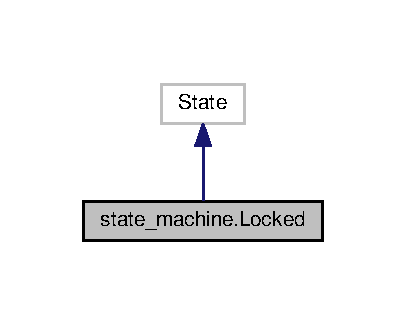
\includegraphics[width=195pt]{classstate__machine_1_1Locked__inherit__graph}
\end{center}
\end{figure}


Collaboration diagram for state\+\_\+machine.\+Locked\+:\nopagebreak
\begin{figure}[H]
\begin{center}
\leavevmode
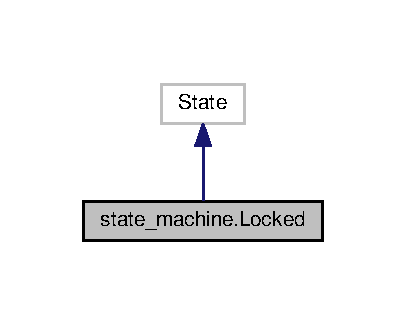
\includegraphics[width=195pt]{classstate__machine_1_1Locked__coll__graph}
\end{center}
\end{figure}
\subsection*{Public Member Functions}
\begin{DoxyCompactItemize}
\item 
def \hyperlink{classstate__machine_1_1Locked_a9b4ed5583dd109a846e88c4ee296dd6a}{\+\_\+\+\_\+init\+\_\+\+\_\+} (self)
\item 
def \hyperlink{classstate__machine_1_1Locked_a9a53fcb4569ca96d6f72d256b112ad5b}{execute} (self, userdata)
\end{DoxyCompactItemize}
\subsection*{Public Attributes}
\begin{DoxyCompactItemize}
\item 
\hyperlink{classstate__machine_1_1Locked_af607507989a4d5039974490e8abada1a}{sensor\+\_\+input}
\item 
\hyperlink{classstate__machine_1_1Locked_a667605824c2d371f1a62b18280a29a02}{rate}
\end{DoxyCompactItemize}


\subsection{Constructor \& Destructor Documentation}
\index{state\+\_\+machine\+::\+Locked@{state\+\_\+machine\+::\+Locked}!\+\_\+\+\_\+init\+\_\+\+\_\+@{\+\_\+\+\_\+init\+\_\+\+\_\+}}
\index{\+\_\+\+\_\+init\+\_\+\+\_\+@{\+\_\+\+\_\+init\+\_\+\+\_\+}!state\+\_\+machine\+::\+Locked@{state\+\_\+machine\+::\+Locked}}
\subsubsection[{\texorpdfstring{\+\_\+\+\_\+init\+\_\+\+\_\+(self)}{__init__(self)}}]{\setlength{\rightskip}{0pt plus 5cm}def state\+\_\+machine.\+Locked.\+\_\+\+\_\+init\+\_\+\+\_\+ (
\begin{DoxyParamCaption}
\item[{}]{self}
\end{DoxyParamCaption}
)}\hypertarget{classstate__machine_1_1Locked_a9b4ed5583dd109a846e88c4ee296dd6a}{}\label{classstate__machine_1_1Locked_a9b4ed5583dd109a846e88c4ee296dd6a}


\subsection{Member Function Documentation}
\index{state\+\_\+machine\+::\+Locked@{state\+\_\+machine\+::\+Locked}!execute@{execute}}
\index{execute@{execute}!state\+\_\+machine\+::\+Locked@{state\+\_\+machine\+::\+Locked}}
\subsubsection[{\texorpdfstring{execute(self, userdata)}{execute(self, userdata)}}]{\setlength{\rightskip}{0pt plus 5cm}def state\+\_\+machine.\+Locked.\+execute (
\begin{DoxyParamCaption}
\item[{}]{self, }
\item[{}]{userdata}
\end{DoxyParamCaption}
)}\hypertarget{classstate__machine_1_1Locked_a9a53fcb4569ca96d6f72d256b112ad5b}{}\label{classstate__machine_1_1Locked_a9a53fcb4569ca96d6f72d256b112ad5b}


\subsection{Member Data Documentation}
\index{state\+\_\+machine\+::\+Locked@{state\+\_\+machine\+::\+Locked}!rate@{rate}}
\index{rate@{rate}!state\+\_\+machine\+::\+Locked@{state\+\_\+machine\+::\+Locked}}
\subsubsection[{\texorpdfstring{rate}{rate}}]{\setlength{\rightskip}{0pt plus 5cm}state\+\_\+machine.\+Locked.\+rate}\hypertarget{classstate__machine_1_1Locked_a667605824c2d371f1a62b18280a29a02}{}\label{classstate__machine_1_1Locked_a667605824c2d371f1a62b18280a29a02}
\index{state\+\_\+machine\+::\+Locked@{state\+\_\+machine\+::\+Locked}!sensor\+\_\+input@{sensor\+\_\+input}}
\index{sensor\+\_\+input@{sensor\+\_\+input}!state\+\_\+machine\+::\+Locked@{state\+\_\+machine\+::\+Locked}}
\subsubsection[{\texorpdfstring{sensor\+\_\+input}{sensor_input}}]{\setlength{\rightskip}{0pt plus 5cm}state\+\_\+machine.\+Locked.\+sensor\+\_\+input}\hypertarget{classstate__machine_1_1Locked_af607507989a4d5039974490e8abada1a}{}\label{classstate__machine_1_1Locked_af607507989a4d5039974490e8abada1a}


The documentation for this class was generated from the following file\+:\begin{DoxyCompactItemize}
\item 
/home/francesco/experimental\+\_\+ws/src/assignment1/src/\hyperlink{state__machine_8py}{state\+\_\+machine.\+py}\end{DoxyCompactItemize}

\hypertarget{classFSM_1_1Normal}{}\section{F\+S\+M.\+Normal Class Reference}
\label{classFSM_1_1Normal}\index{F\+S\+M.\+Normal@{F\+S\+M.\+Normal}}


Inheritance diagram for F\+S\+M.\+Normal\+:\nopagebreak
\begin{figure}[H]
\begin{center}
\leavevmode
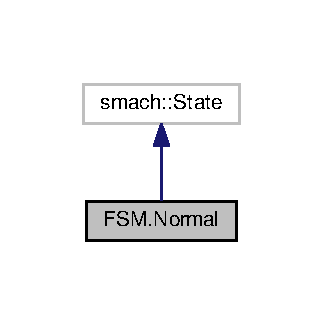
\includegraphics[width=155pt]{classFSM_1_1Normal__inherit__graph}
\end{center}
\end{figure}


Collaboration diagram for F\+S\+M.\+Normal\+:\nopagebreak
\begin{figure}[H]
\begin{center}
\leavevmode
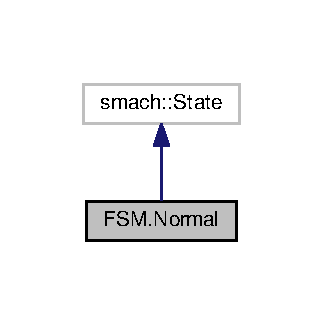
\includegraphics[width=155pt]{classFSM_1_1Normal__coll__graph}
\end{center}
\end{figure}
\subsection*{Public Member Functions}
\begin{DoxyCompactItemize}
\item 
def \hyperlink{classFSM_1_1Normal_a21e63c972c3a4b1417c60b5d18ea18bd}{\+\_\+\+\_\+init\+\_\+\+\_\+} (self)
\item 
def \hyperlink{classFSM_1_1Normal_ae85b3201d4649dac559f39d327f76f6e}{execute} (self, userdata)
\end{DoxyCompactItemize}
\subsection*{Public Attributes}
\begin{DoxyCompactItemize}
\item 
\hyperlink{classFSM_1_1Normal_a99ce5b8dddfae4e6a49f4c1d292b5d83}{rate}
\item 
\hyperlink{classFSM_1_1Normal_aeeb78ed66cc617acb7ac428aa2507b6d}{counter}
\end{DoxyCompactItemize}


\subsection{Constructor \& Destructor Documentation}
\index{F\+S\+M\+::\+Normal@{F\+S\+M\+::\+Normal}!\+\_\+\+\_\+init\+\_\+\+\_\+@{\+\_\+\+\_\+init\+\_\+\+\_\+}}
\index{\+\_\+\+\_\+init\+\_\+\+\_\+@{\+\_\+\+\_\+init\+\_\+\+\_\+}!F\+S\+M\+::\+Normal@{F\+S\+M\+::\+Normal}}
\subsubsection[{\texorpdfstring{\+\_\+\+\_\+init\+\_\+\+\_\+(self)}{__init__(self)}}]{\setlength{\rightskip}{0pt plus 5cm}def F\+S\+M.\+Normal.\+\_\+\+\_\+init\+\_\+\+\_\+ (
\begin{DoxyParamCaption}
\item[{}]{self}
\end{DoxyParamCaption}
)}\hypertarget{classFSM_1_1Normal_a21e63c972c3a4b1417c60b5d18ea18bd}{}\label{classFSM_1_1Normal_a21e63c972c3a4b1417c60b5d18ea18bd}


\subsection{Member Function Documentation}
\index{F\+S\+M\+::\+Normal@{F\+S\+M\+::\+Normal}!execute@{execute}}
\index{execute@{execute}!F\+S\+M\+::\+Normal@{F\+S\+M\+::\+Normal}}
\subsubsection[{\texorpdfstring{execute(self, userdata)}{execute(self, userdata)}}]{\setlength{\rightskip}{0pt plus 5cm}def F\+S\+M.\+Normal.\+execute (
\begin{DoxyParamCaption}
\item[{}]{self, }
\item[{}]{userdata}
\end{DoxyParamCaption}
)}\hypertarget{classFSM_1_1Normal_ae85b3201d4649dac559f39d327f76f6e}{}\label{classFSM_1_1Normal_ae85b3201d4649dac559f39d327f76f6e}


\subsection{Member Data Documentation}
\index{F\+S\+M\+::\+Normal@{F\+S\+M\+::\+Normal}!counter@{counter}}
\index{counter@{counter}!F\+S\+M\+::\+Normal@{F\+S\+M\+::\+Normal}}
\subsubsection[{\texorpdfstring{counter}{counter}}]{\setlength{\rightskip}{0pt plus 5cm}F\+S\+M.\+Normal.\+counter}\hypertarget{classFSM_1_1Normal_aeeb78ed66cc617acb7ac428aa2507b6d}{}\label{classFSM_1_1Normal_aeeb78ed66cc617acb7ac428aa2507b6d}
\index{F\+S\+M\+::\+Normal@{F\+S\+M\+::\+Normal}!rate@{rate}}
\index{rate@{rate}!F\+S\+M\+::\+Normal@{F\+S\+M\+::\+Normal}}
\subsubsection[{\texorpdfstring{rate}{rate}}]{\setlength{\rightskip}{0pt plus 5cm}F\+S\+M.\+Normal.\+rate}\hypertarget{classFSM_1_1Normal_a99ce5b8dddfae4e6a49f4c1d292b5d83}{}\label{classFSM_1_1Normal_a99ce5b8dddfae4e6a49f4c1d292b5d83}


The documentation for this class was generated from the following file\+:\begin{DoxyCompactItemize}
\item 
/home/francesco/experimental\+\_\+ws/src/assignment1/src/\hyperlink{FSM_8py}{F\+S\+M.\+py}\end{DoxyCompactItemize}

\hypertarget{classFSMplay_1_1Normal}{}\section{F\+S\+Mplay.\+Normal Class Reference}
\label{classFSMplay_1_1Normal}\index{F\+S\+Mplay.\+Normal@{F\+S\+Mplay.\+Normal}}


Inheritance diagram for F\+S\+Mplay.\+Normal\+:\nopagebreak
\begin{figure}[H]
\begin{center}
\leavevmode
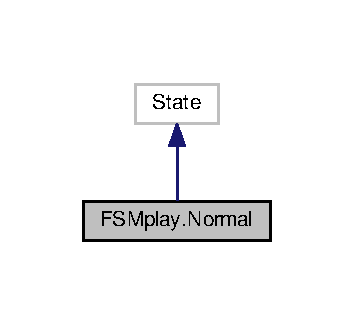
\includegraphics[width=170pt]{classFSMplay_1_1Normal__inherit__graph}
\end{center}
\end{figure}


Collaboration diagram for F\+S\+Mplay.\+Normal\+:\nopagebreak
\begin{figure}[H]
\begin{center}
\leavevmode
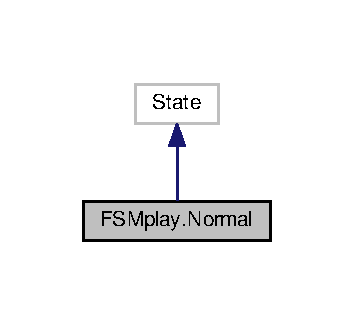
\includegraphics[width=170pt]{classFSMplay_1_1Normal__coll__graph}
\end{center}
\end{figure}
\subsection*{Public Member Functions}
\begin{DoxyCompactItemize}
\item 
def \hyperlink{classFSMplay_1_1Normal_a02206ed7d99445b42a37574de2237f34}{\+\_\+\+\_\+init\+\_\+\+\_\+} (self)
\item 
def \hyperlink{classFSMplay_1_1Normal_a3792bdd0853c6220c716d6bc9c73d810}{execute} (self, userdata)
\end{DoxyCompactItemize}
\subsection*{Public Attributes}
\begin{DoxyCompactItemize}
\item 
\hyperlink{classFSMplay_1_1Normal_a62273aa35f449d8636797ce21dfd2aa2}{rate}
\item 
\hyperlink{classFSMplay_1_1Normal_acbb61a2d3f054bd0e50ee54ba2c910c0}{counter}
\end{DoxyCompactItemize}


\subsection{Constructor \& Destructor Documentation}
\index{F\+S\+Mplay\+::\+Normal@{F\+S\+Mplay\+::\+Normal}!\+\_\+\+\_\+init\+\_\+\+\_\+@{\+\_\+\+\_\+init\+\_\+\+\_\+}}
\index{\+\_\+\+\_\+init\+\_\+\+\_\+@{\+\_\+\+\_\+init\+\_\+\+\_\+}!F\+S\+Mplay\+::\+Normal@{F\+S\+Mplay\+::\+Normal}}
\subsubsection[{\texorpdfstring{\+\_\+\+\_\+init\+\_\+\+\_\+(self)}{__init__(self)}}]{\setlength{\rightskip}{0pt plus 5cm}def F\+S\+Mplay.\+Normal.\+\_\+\+\_\+init\+\_\+\+\_\+ (
\begin{DoxyParamCaption}
\item[{}]{self}
\end{DoxyParamCaption}
)}\hypertarget{classFSMplay_1_1Normal_a02206ed7d99445b42a37574de2237f34}{}\label{classFSMplay_1_1Normal_a02206ed7d99445b42a37574de2237f34}


\subsection{Member Function Documentation}
\index{F\+S\+Mplay\+::\+Normal@{F\+S\+Mplay\+::\+Normal}!execute@{execute}}
\index{execute@{execute}!F\+S\+Mplay\+::\+Normal@{F\+S\+Mplay\+::\+Normal}}
\subsubsection[{\texorpdfstring{execute(self, userdata)}{execute(self, userdata)}}]{\setlength{\rightskip}{0pt plus 5cm}def F\+S\+Mplay.\+Normal.\+execute (
\begin{DoxyParamCaption}
\item[{}]{self, }
\item[{}]{userdata}
\end{DoxyParamCaption}
)}\hypertarget{classFSMplay_1_1Normal_a3792bdd0853c6220c716d6bc9c73d810}{}\label{classFSMplay_1_1Normal_a3792bdd0853c6220c716d6bc9c73d810}


\subsection{Member Data Documentation}
\index{F\+S\+Mplay\+::\+Normal@{F\+S\+Mplay\+::\+Normal}!counter@{counter}}
\index{counter@{counter}!F\+S\+Mplay\+::\+Normal@{F\+S\+Mplay\+::\+Normal}}
\subsubsection[{\texorpdfstring{counter}{counter}}]{\setlength{\rightskip}{0pt plus 5cm}F\+S\+Mplay.\+Normal.\+counter}\hypertarget{classFSMplay_1_1Normal_acbb61a2d3f054bd0e50ee54ba2c910c0}{}\label{classFSMplay_1_1Normal_acbb61a2d3f054bd0e50ee54ba2c910c0}
\index{F\+S\+Mplay\+::\+Normal@{F\+S\+Mplay\+::\+Normal}!rate@{rate}}
\index{rate@{rate}!F\+S\+Mplay\+::\+Normal@{F\+S\+Mplay\+::\+Normal}}
\subsubsection[{\texorpdfstring{rate}{rate}}]{\setlength{\rightskip}{0pt plus 5cm}F\+S\+Mplay.\+Normal.\+rate}\hypertarget{classFSMplay_1_1Normal_a62273aa35f449d8636797ce21dfd2aa2}{}\label{classFSMplay_1_1Normal_a62273aa35f449d8636797ce21dfd2aa2}


The documentation for this class was generated from the following file\+:\begin{DoxyCompactItemize}
\item 
/home/francesco/experimental\+\_\+ws/src/assignment1/src/\hyperlink{FSMplay_8py}{F\+S\+Mplay.\+py}\end{DoxyCompactItemize}

\hypertarget{classFSM_1_1Play}{}\section{F\+S\+M.\+Play Class Reference}
\label{classFSM_1_1Play}\index{F\+S\+M.\+Play@{F\+S\+M.\+Play}}


defines the P\+L\+AY state  




Inheritance diagram for F\+S\+M.\+Play\+:\nopagebreak
\begin{figure}[H]
\begin{center}
\leavevmode
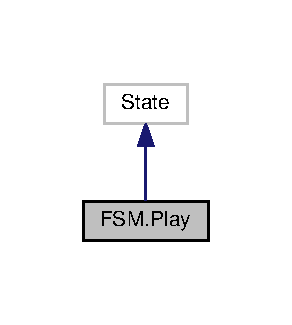
\includegraphics[width=140pt]{classFSM_1_1Play__inherit__graph}
\end{center}
\end{figure}


Collaboration diagram for F\+S\+M.\+Play\+:\nopagebreak
\begin{figure}[H]
\begin{center}
\leavevmode
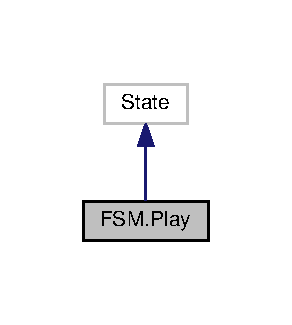
\includegraphics[width=140pt]{classFSM_1_1Play__coll__graph}
\end{center}
\end{figure}
\subsection*{Public Member Functions}
\begin{DoxyCompactItemize}
\item 
def \hyperlink{classFSM_1_1Play_adbcc8a351d8013f0fd40e778bc85b5e0}{\+\_\+\+\_\+init\+\_\+\+\_\+} (self)
\item 
def \hyperlink{classFSM_1_1Play_ab7c062e30152b05f18bccd330d618634}{execute} (self, userdata)
\end{DoxyCompactItemize}
\subsection*{Public Attributes}
\begin{DoxyCompactItemize}
\item 
\hyperlink{classFSM_1_1Play_a8aea6272cf59d81e990b67d6b62c84ac}{sensor\+\_\+input}
\item 
\hyperlink{classFSM_1_1Play_a21dea0882a6b4f29db67e50234b0f168}{rate}
\end{DoxyCompactItemize}


\subsection{Detailed Description}
defines the P\+L\+AY state 

\subsection{Constructor \& Destructor Documentation}
\index{F\+S\+M\+::\+Play@{F\+S\+M\+::\+Play}!\+\_\+\+\_\+init\+\_\+\+\_\+@{\+\_\+\+\_\+init\+\_\+\+\_\+}}
\index{\+\_\+\+\_\+init\+\_\+\+\_\+@{\+\_\+\+\_\+init\+\_\+\+\_\+}!F\+S\+M\+::\+Play@{F\+S\+M\+::\+Play}}
\subsubsection[{\texorpdfstring{\+\_\+\+\_\+init\+\_\+\+\_\+(self)}{__init__(self)}}]{\setlength{\rightskip}{0pt plus 5cm}def F\+S\+M.\+Play.\+\_\+\+\_\+init\+\_\+\+\_\+ (
\begin{DoxyParamCaption}
\item[{}]{self}
\end{DoxyParamCaption}
)}\hypertarget{classFSM_1_1Play_adbcc8a351d8013f0fd40e778bc85b5e0}{}\label{classFSM_1_1Play_adbcc8a351d8013f0fd40e778bc85b5e0}


\subsection{Member Function Documentation}
\index{F\+S\+M\+::\+Play@{F\+S\+M\+::\+Play}!execute@{execute}}
\index{execute@{execute}!F\+S\+M\+::\+Play@{F\+S\+M\+::\+Play}}
\subsubsection[{\texorpdfstring{execute(self, userdata)}{execute(self, userdata)}}]{\setlength{\rightskip}{0pt plus 5cm}def F\+S\+M.\+Play.\+execute (
\begin{DoxyParamCaption}
\item[{}]{self, }
\item[{}]{userdata}
\end{DoxyParamCaption}
)}\hypertarget{classFSM_1_1Play_ab7c062e30152b05f18bccd330d618634}{}\label{classFSM_1_1Play_ab7c062e30152b05f18bccd330d618634}


\subsection{Member Data Documentation}
\index{F\+S\+M\+::\+Play@{F\+S\+M\+::\+Play}!rate@{rate}}
\index{rate@{rate}!F\+S\+M\+::\+Play@{F\+S\+M\+::\+Play}}
\subsubsection[{\texorpdfstring{rate}{rate}}]{\setlength{\rightskip}{0pt plus 5cm}F\+S\+M.\+Play.\+rate}\hypertarget{classFSM_1_1Play_a21dea0882a6b4f29db67e50234b0f168}{}\label{classFSM_1_1Play_a21dea0882a6b4f29db67e50234b0f168}
\index{F\+S\+M\+::\+Play@{F\+S\+M\+::\+Play}!sensor\+\_\+input@{sensor\+\_\+input}}
\index{sensor\+\_\+input@{sensor\+\_\+input}!F\+S\+M\+::\+Play@{F\+S\+M\+::\+Play}}
\subsubsection[{\texorpdfstring{sensor\+\_\+input}{sensor_input}}]{\setlength{\rightskip}{0pt plus 5cm}F\+S\+M.\+Play.\+sensor\+\_\+input}\hypertarget{classFSM_1_1Play_a8aea6272cf59d81e990b67d6b62c84ac}{}\label{classFSM_1_1Play_a8aea6272cf59d81e990b67d6b62c84ac}


The documentation for this class was generated from the following file\+:\begin{DoxyCompactItemize}
\item 
/home/francesco/experimental\+\_\+ws/src/assignment1/src/\hyperlink{FSM_8py}{F\+S\+M.\+py}\end{DoxyCompactItemize}

\hypertarget{classFSMplay_1_1Play}{}\section{F\+S\+Mplay.\+Play Class Reference}
\label{classFSMplay_1_1Play}\index{F\+S\+Mplay.\+Play@{F\+S\+Mplay.\+Play}}


Inheritance diagram for F\+S\+Mplay.\+Play\+:\nopagebreak
\begin{figure}[H]
\begin{center}
\leavevmode
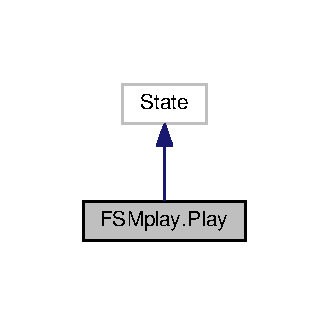
\includegraphics[width=158pt]{classFSMplay_1_1Play__inherit__graph}
\end{center}
\end{figure}


Collaboration diagram for F\+S\+Mplay.\+Play\+:\nopagebreak
\begin{figure}[H]
\begin{center}
\leavevmode
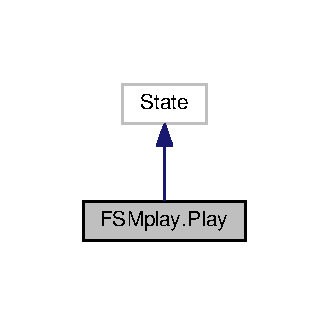
\includegraphics[width=158pt]{classFSMplay_1_1Play__coll__graph}
\end{center}
\end{figure}
\subsection*{Public Member Functions}
\begin{DoxyCompactItemize}
\item 
def \hyperlink{classFSMplay_1_1Play_a9f4e0fb04109cac88a2f0f498b7c3b55}{\+\_\+\+\_\+init\+\_\+\+\_\+} (self)
\item 
def \hyperlink{classFSMplay_1_1Play_a699a762c4344fc54a6fc97a20c0f604d}{execute} (self, userdata)
\end{DoxyCompactItemize}
\subsection*{Public Attributes}
\begin{DoxyCompactItemize}
\item 
\hyperlink{classFSMplay_1_1Play_a01e386e2402ae9ae8a3dcf475d8ce180}{sensor\+\_\+input}
\item 
\hyperlink{classFSMplay_1_1Play_ad0f5331aa8db5087e451db135bd9e1d8}{rate}
\end{DoxyCompactItemize}


\subsection{Constructor \& Destructor Documentation}
\index{F\+S\+Mplay\+::\+Play@{F\+S\+Mplay\+::\+Play}!\+\_\+\+\_\+init\+\_\+\+\_\+@{\+\_\+\+\_\+init\+\_\+\+\_\+}}
\index{\+\_\+\+\_\+init\+\_\+\+\_\+@{\+\_\+\+\_\+init\+\_\+\+\_\+}!F\+S\+Mplay\+::\+Play@{F\+S\+Mplay\+::\+Play}}
\subsubsection[{\texorpdfstring{\+\_\+\+\_\+init\+\_\+\+\_\+(self)}{__init__(self)}}]{\setlength{\rightskip}{0pt plus 5cm}def F\+S\+Mplay.\+Play.\+\_\+\+\_\+init\+\_\+\+\_\+ (
\begin{DoxyParamCaption}
\item[{}]{self}
\end{DoxyParamCaption}
)}\hypertarget{classFSMplay_1_1Play_a9f4e0fb04109cac88a2f0f498b7c3b55}{}\label{classFSMplay_1_1Play_a9f4e0fb04109cac88a2f0f498b7c3b55}


\subsection{Member Function Documentation}
\index{F\+S\+Mplay\+::\+Play@{F\+S\+Mplay\+::\+Play}!execute@{execute}}
\index{execute@{execute}!F\+S\+Mplay\+::\+Play@{F\+S\+Mplay\+::\+Play}}
\subsubsection[{\texorpdfstring{execute(self, userdata)}{execute(self, userdata)}}]{\setlength{\rightskip}{0pt plus 5cm}def F\+S\+Mplay.\+Play.\+execute (
\begin{DoxyParamCaption}
\item[{}]{self, }
\item[{}]{userdata}
\end{DoxyParamCaption}
)}\hypertarget{classFSMplay_1_1Play_a699a762c4344fc54a6fc97a20c0f604d}{}\label{classFSMplay_1_1Play_a699a762c4344fc54a6fc97a20c0f604d}


\subsection{Member Data Documentation}
\index{F\+S\+Mplay\+::\+Play@{F\+S\+Mplay\+::\+Play}!rate@{rate}}
\index{rate@{rate}!F\+S\+Mplay\+::\+Play@{F\+S\+Mplay\+::\+Play}}
\subsubsection[{\texorpdfstring{rate}{rate}}]{\setlength{\rightskip}{0pt plus 5cm}F\+S\+Mplay.\+Play.\+rate}\hypertarget{classFSMplay_1_1Play_ad0f5331aa8db5087e451db135bd9e1d8}{}\label{classFSMplay_1_1Play_ad0f5331aa8db5087e451db135bd9e1d8}
\index{F\+S\+Mplay\+::\+Play@{F\+S\+Mplay\+::\+Play}!sensor\+\_\+input@{sensor\+\_\+input}}
\index{sensor\+\_\+input@{sensor\+\_\+input}!F\+S\+Mplay\+::\+Play@{F\+S\+Mplay\+::\+Play}}
\subsubsection[{\texorpdfstring{sensor\+\_\+input}{sensor_input}}]{\setlength{\rightskip}{0pt plus 5cm}F\+S\+Mplay.\+Play.\+sensor\+\_\+input}\hypertarget{classFSMplay_1_1Play_a01e386e2402ae9ae8a3dcf475d8ce180}{}\label{classFSMplay_1_1Play_a01e386e2402ae9ae8a3dcf475d8ce180}


The documentation for this class was generated from the following file\+:\begin{DoxyCompactItemize}
\item 
/home/francesco/experimental\+\_\+ws/src/assignment1/src/\hyperlink{FSMplay_8py}{F\+S\+Mplay.\+py}\end{DoxyCompactItemize}

\hypertarget{classFSMplay_1_1Sleep}{}\section{F\+S\+Mplay.\+Sleep Class Reference}
\label{classFSMplay_1_1Sleep}\index{F\+S\+Mplay.\+Sleep@{F\+S\+Mplay.\+Sleep}}


Inheritance diagram for F\+S\+Mplay.\+Sleep\+:\nopagebreak
\begin{figure}[H]
\begin{center}
\leavevmode
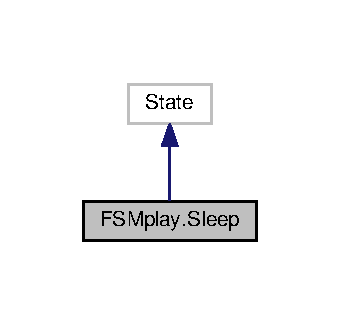
\includegraphics[width=163pt]{classFSMplay_1_1Sleep__inherit__graph}
\end{center}
\end{figure}


Collaboration diagram for F\+S\+Mplay.\+Sleep\+:\nopagebreak
\begin{figure}[H]
\begin{center}
\leavevmode
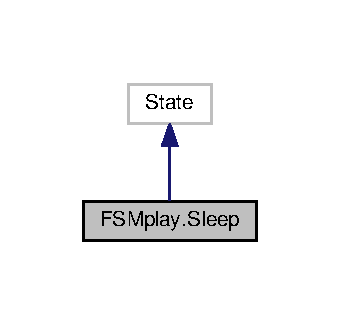
\includegraphics[width=163pt]{classFSMplay_1_1Sleep__coll__graph}
\end{center}
\end{figure}
\subsection*{Public Member Functions}
\begin{DoxyCompactItemize}
\item 
def \hyperlink{classFSMplay_1_1Sleep_afccc38ee1eababdf0f39d5210d18f864}{\+\_\+\+\_\+init\+\_\+\+\_\+} (self)
\item 
def \hyperlink{classFSMplay_1_1Sleep_a39f49b7e0a6cbd4d453d2b9fb365d21c}{execute} (self, userdata)
\end{DoxyCompactItemize}
\subsection*{Public Attributes}
\begin{DoxyCompactItemize}
\item 
\hyperlink{classFSMplay_1_1Sleep_a911ff4d10f330e63ac1d0c34ec2003c3}{sensor\+\_\+input}
\item 
\hyperlink{classFSMplay_1_1Sleep_a85f03dc0ae8811e617eaef79ac9d3835}{rate}
\end{DoxyCompactItemize}


\subsection{Constructor \& Destructor Documentation}
\index{F\+S\+Mplay\+::\+Sleep@{F\+S\+Mplay\+::\+Sleep}!\+\_\+\+\_\+init\+\_\+\+\_\+@{\+\_\+\+\_\+init\+\_\+\+\_\+}}
\index{\+\_\+\+\_\+init\+\_\+\+\_\+@{\+\_\+\+\_\+init\+\_\+\+\_\+}!F\+S\+Mplay\+::\+Sleep@{F\+S\+Mplay\+::\+Sleep}}
\subsubsection[{\texorpdfstring{\+\_\+\+\_\+init\+\_\+\+\_\+(self)}{__init__(self)}}]{\setlength{\rightskip}{0pt plus 5cm}def F\+S\+Mplay.\+Sleep.\+\_\+\+\_\+init\+\_\+\+\_\+ (
\begin{DoxyParamCaption}
\item[{}]{self}
\end{DoxyParamCaption}
)}\hypertarget{classFSMplay_1_1Sleep_afccc38ee1eababdf0f39d5210d18f864}{}\label{classFSMplay_1_1Sleep_afccc38ee1eababdf0f39d5210d18f864}


\subsection{Member Function Documentation}
\index{F\+S\+Mplay\+::\+Sleep@{F\+S\+Mplay\+::\+Sleep}!execute@{execute}}
\index{execute@{execute}!F\+S\+Mplay\+::\+Sleep@{F\+S\+Mplay\+::\+Sleep}}
\subsubsection[{\texorpdfstring{execute(self, userdata)}{execute(self, userdata)}}]{\setlength{\rightskip}{0pt plus 5cm}def F\+S\+Mplay.\+Sleep.\+execute (
\begin{DoxyParamCaption}
\item[{}]{self, }
\item[{}]{userdata}
\end{DoxyParamCaption}
)}\hypertarget{classFSMplay_1_1Sleep_a39f49b7e0a6cbd4d453d2b9fb365d21c}{}\label{classFSMplay_1_1Sleep_a39f49b7e0a6cbd4d453d2b9fb365d21c}


\subsection{Member Data Documentation}
\index{F\+S\+Mplay\+::\+Sleep@{F\+S\+Mplay\+::\+Sleep}!rate@{rate}}
\index{rate@{rate}!F\+S\+Mplay\+::\+Sleep@{F\+S\+Mplay\+::\+Sleep}}
\subsubsection[{\texorpdfstring{rate}{rate}}]{\setlength{\rightskip}{0pt plus 5cm}F\+S\+Mplay.\+Sleep.\+rate}\hypertarget{classFSMplay_1_1Sleep_a85f03dc0ae8811e617eaef79ac9d3835}{}\label{classFSMplay_1_1Sleep_a85f03dc0ae8811e617eaef79ac9d3835}
\index{F\+S\+Mplay\+::\+Sleep@{F\+S\+Mplay\+::\+Sleep}!sensor\+\_\+input@{sensor\+\_\+input}}
\index{sensor\+\_\+input@{sensor\+\_\+input}!F\+S\+Mplay\+::\+Sleep@{F\+S\+Mplay\+::\+Sleep}}
\subsubsection[{\texorpdfstring{sensor\+\_\+input}{sensor_input}}]{\setlength{\rightskip}{0pt plus 5cm}F\+S\+Mplay.\+Sleep.\+sensor\+\_\+input}\hypertarget{classFSMplay_1_1Sleep_a911ff4d10f330e63ac1d0c34ec2003c3}{}\label{classFSMplay_1_1Sleep_a911ff4d10f330e63ac1d0c34ec2003c3}


The documentation for this class was generated from the following file\+:\begin{DoxyCompactItemize}
\item 
/home/francesco/experimental\+\_\+ws/src/assignment1/src/\hyperlink{FSMplay_8py}{F\+S\+Mplay.\+py}\end{DoxyCompactItemize}

\hypertarget{classFSM_1_1Sleep}{}\section{F\+S\+M.\+Sleep Class Reference}
\label{classFSM_1_1Sleep}\index{F\+S\+M.\+Sleep@{F\+S\+M.\+Sleep}}


Inheritance diagram for F\+S\+M.\+Sleep\+:\nopagebreak
\begin{figure}[H]
\begin{center}
\leavevmode
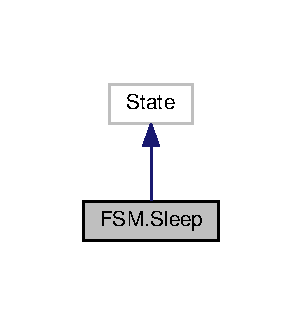
\includegraphics[width=145pt]{classFSM_1_1Sleep__inherit__graph}
\end{center}
\end{figure}


Collaboration diagram for F\+S\+M.\+Sleep\+:\nopagebreak
\begin{figure}[H]
\begin{center}
\leavevmode
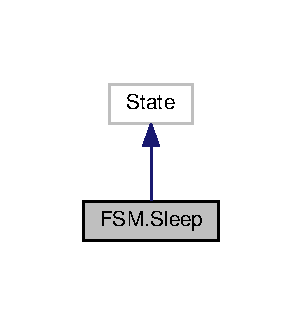
\includegraphics[width=145pt]{classFSM_1_1Sleep__coll__graph}
\end{center}
\end{figure}
\subsection*{Public Member Functions}
\begin{DoxyCompactItemize}
\item 
def \hyperlink{classFSM_1_1Sleep_a54af482c09a00a2c1624fba609c4f780}{\+\_\+\+\_\+init\+\_\+\+\_\+} (self)
\item 
def \hyperlink{classFSM_1_1Sleep_ad9e21d03aeeb758686055fb3ca68a639}{execute} (self, userdata)
\end{DoxyCompactItemize}
\subsection*{Public Attributes}
\begin{DoxyCompactItemize}
\item 
\hyperlink{classFSM_1_1Sleep_ae09e7c57423ebb912d192c709faa3c01}{rate}
\end{DoxyCompactItemize}


\subsection{Constructor \& Destructor Documentation}
\index{F\+S\+M\+::\+Sleep@{F\+S\+M\+::\+Sleep}!\+\_\+\+\_\+init\+\_\+\+\_\+@{\+\_\+\+\_\+init\+\_\+\+\_\+}}
\index{\+\_\+\+\_\+init\+\_\+\+\_\+@{\+\_\+\+\_\+init\+\_\+\+\_\+}!F\+S\+M\+::\+Sleep@{F\+S\+M\+::\+Sleep}}
\subsubsection[{\texorpdfstring{\+\_\+\+\_\+init\+\_\+\+\_\+(self)}{__init__(self)}}]{\setlength{\rightskip}{0pt plus 5cm}def F\+S\+M.\+Sleep.\+\_\+\+\_\+init\+\_\+\+\_\+ (
\begin{DoxyParamCaption}
\item[{}]{self}
\end{DoxyParamCaption}
)}\hypertarget{classFSM_1_1Sleep_a54af482c09a00a2c1624fba609c4f780}{}\label{classFSM_1_1Sleep_a54af482c09a00a2c1624fba609c4f780}


\subsection{Member Function Documentation}
\index{F\+S\+M\+::\+Sleep@{F\+S\+M\+::\+Sleep}!execute@{execute}}
\index{execute@{execute}!F\+S\+M\+::\+Sleep@{F\+S\+M\+::\+Sleep}}
\subsubsection[{\texorpdfstring{execute(self, userdata)}{execute(self, userdata)}}]{\setlength{\rightskip}{0pt plus 5cm}def F\+S\+M.\+Sleep.\+execute (
\begin{DoxyParamCaption}
\item[{}]{self, }
\item[{}]{userdata}
\end{DoxyParamCaption}
)}\hypertarget{classFSM_1_1Sleep_ad9e21d03aeeb758686055fb3ca68a639}{}\label{classFSM_1_1Sleep_ad9e21d03aeeb758686055fb3ca68a639}


\subsection{Member Data Documentation}
\index{F\+S\+M\+::\+Sleep@{F\+S\+M\+::\+Sleep}!rate@{rate}}
\index{rate@{rate}!F\+S\+M\+::\+Sleep@{F\+S\+M\+::\+Sleep}}
\subsubsection[{\texorpdfstring{rate}{rate}}]{\setlength{\rightskip}{0pt plus 5cm}F\+S\+M.\+Sleep.\+rate}\hypertarget{classFSM_1_1Sleep_ae09e7c57423ebb912d192c709faa3c01}{}\label{classFSM_1_1Sleep_ae09e7c57423ebb912d192c709faa3c01}


The documentation for this class was generated from the following file\+:\begin{DoxyCompactItemize}
\item 
/home/francesco/experimental\+\_\+ws/src/assignment1/src/\hyperlink{FSM_8py}{F\+S\+M.\+py}\end{DoxyCompactItemize}

\hypertarget{classstate__machine_1_1Unlocked}{}\section{state\+\_\+machine.\+Unlocked Class Reference}
\label{classstate__machine_1_1Unlocked}\index{state\+\_\+machine.\+Unlocked@{state\+\_\+machine.\+Unlocked}}


Inheritance diagram for state\+\_\+machine.\+Unlocked\+:\nopagebreak
\begin{figure}[H]
\begin{center}
\leavevmode
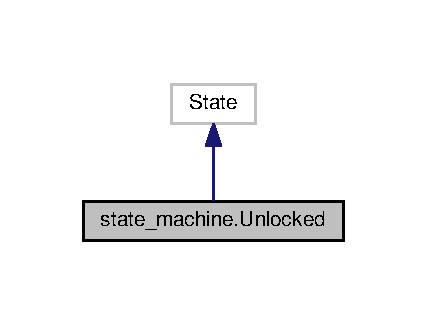
\includegraphics[width=205pt]{classstate__machine_1_1Unlocked__inherit__graph}
\end{center}
\end{figure}


Collaboration diagram for state\+\_\+machine.\+Unlocked\+:\nopagebreak
\begin{figure}[H]
\begin{center}
\leavevmode
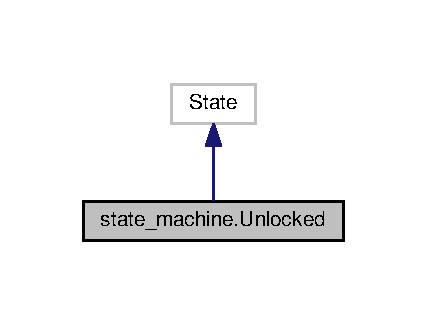
\includegraphics[width=205pt]{classstate__machine_1_1Unlocked__coll__graph}
\end{center}
\end{figure}
\subsection*{Public Member Functions}
\begin{DoxyCompactItemize}
\item 
def \hyperlink{classstate__machine_1_1Unlocked_a98fc7d3f4e0e121b3680ce2ef7c981aa}{\+\_\+\+\_\+init\+\_\+\+\_\+} (self)
\item 
def \hyperlink{classstate__machine_1_1Unlocked_aedea4a1195c913739a334981ff6ccca5}{execute} (self, userdata)
\end{DoxyCompactItemize}


\subsection{Constructor \& Destructor Documentation}
\index{state\+\_\+machine\+::\+Unlocked@{state\+\_\+machine\+::\+Unlocked}!\+\_\+\+\_\+init\+\_\+\+\_\+@{\+\_\+\+\_\+init\+\_\+\+\_\+}}
\index{\+\_\+\+\_\+init\+\_\+\+\_\+@{\+\_\+\+\_\+init\+\_\+\+\_\+}!state\+\_\+machine\+::\+Unlocked@{state\+\_\+machine\+::\+Unlocked}}
\subsubsection[{\texorpdfstring{\+\_\+\+\_\+init\+\_\+\+\_\+(self)}{__init__(self)}}]{\setlength{\rightskip}{0pt plus 5cm}def state\+\_\+machine.\+Unlocked.\+\_\+\+\_\+init\+\_\+\+\_\+ (
\begin{DoxyParamCaption}
\item[{}]{self}
\end{DoxyParamCaption}
)}\hypertarget{classstate__machine_1_1Unlocked_a98fc7d3f4e0e121b3680ce2ef7c981aa}{}\label{classstate__machine_1_1Unlocked_a98fc7d3f4e0e121b3680ce2ef7c981aa}


\subsection{Member Function Documentation}
\index{state\+\_\+machine\+::\+Unlocked@{state\+\_\+machine\+::\+Unlocked}!execute@{execute}}
\index{execute@{execute}!state\+\_\+machine\+::\+Unlocked@{state\+\_\+machine\+::\+Unlocked}}
\subsubsection[{\texorpdfstring{execute(self, userdata)}{execute(self, userdata)}}]{\setlength{\rightskip}{0pt plus 5cm}def state\+\_\+machine.\+Unlocked.\+execute (
\begin{DoxyParamCaption}
\item[{}]{self, }
\item[{}]{userdata}
\end{DoxyParamCaption}
)}\hypertarget{classstate__machine_1_1Unlocked_aedea4a1195c913739a334981ff6ccca5}{}\label{classstate__machine_1_1Unlocked_aedea4a1195c913739a334981ff6ccca5}


The documentation for this class was generated from the following file\+:\begin{DoxyCompactItemize}
\item 
/home/francesco/experimental\+\_\+ws/src/assignment1/src/\hyperlink{state__machine_8py}{state\+\_\+machine.\+py}\end{DoxyCompactItemize}

\chapter{File Documentation}
\hypertarget{commandManager_8py}{}\section{/home/francescotesta/experimental\+\_\+ws/src/final\+\_\+assignment/scripts/command\+Manager.py File Reference}
\label{commandManager_8py}\index{/home/francescotesta/experimental\+\_\+ws/src/final\+\_\+assignment/scripts/command\+Manager.\+py@{/home/francescotesta/experimental\+\_\+ws/src/final\+\_\+assignment/scripts/command\+Manager.\+py}}


This script is a node which is the core of the entier project.  


\subsection*{Classes}
\begin{DoxyCompactItemize}
\item 
class \hyperlink{classcommandManager_1_1Normal}{command\+Manager.\+Normal}
\item 
class \hyperlink{classcommandManager_1_1Sleep}{command\+Manager.\+Sleep}
\item 
class \hyperlink{classcommandManager_1_1Play}{command\+Manager.\+Play}
\item 
class \hyperlink{classcommandManager_1_1Track}{command\+Manager.\+Track}
\item 
class \hyperlink{classcommandManager_1_1Find}{command\+Manager.\+Find}
\end{DoxyCompactItemize}
\subsection*{Namespaces}
\begin{DoxyCompactItemize}
\item 
 \hyperlink{namespacecommandManager}{command\+Manager}
\end{DoxyCompactItemize}
\subsection*{Functions}
\begin{DoxyCompactItemize}
\item 
def \hyperlink{namespacecommandManager_a2310383d56755f0a09a75b1a92130e21}{command\+Manager.\+U\+Icallback} (data)
\begin{DoxyCompactList}\small\item\em Callback mathod of the U\+Isubscriber which handels the commands sent by the user. \end{DoxyCompactList}\item 
def \hyperlink{namespacecommandManager_aa96fd2ed94c8c1168e09ced4015dcb1b}{command\+Manager.\+new\+Room\+Detected} (color)
\begin{DoxyCompactList}\small\item\em Callback function of the new\+Room\+Sub subscriber which recives the color of the new detected room. \end{DoxyCompactList}\item 
def \hyperlink{namespacecommandManager_af8e54858c65310eb1e131529bf200516}{command\+Manager.\+move\+\_\+base\+\_\+go\+\_\+to} (x, y)
\begin{DoxyCompactList}\small\item\em Method which prepares and send the goal to the move\+\_\+base action server. \end{DoxyCompactList}\item 
def \hyperlink{namespacecommandManager_ae8b570eb4bf393859bc74c9cb5fe125f}{command\+Manager.\+main} ()
\end{DoxyCompactItemize}
\subsection*{Variables}
\begin{DoxyCompactItemize}
\item 
dictionary \hyperlink{namespacecommandManager_a3c82d03952562f9cf96be2e80ae059a3}{command\+Manager.\+control\+\_\+variables}
\begin{DoxyCompactList}\small\item\em Dictionary which contains flags and global variables. \end{DoxyCompactList}\item 
\hyperlink{namespacecommandManager_ad81f5cdd9bf18b67989c77a2329b9e28}{command\+Manager.\+client} = actionlib.\+Simple\+Action\+Client(\textquotesingle{}move\+\_\+base\textquotesingle{},Move\+Base\+Action)
\begin{DoxyCompactList}\small\item\em Initialization of the move\+\_\+base client in order to assign target position to the move\+\_\+base action server. \end{DoxyCompactList}\item 
\hyperlink{namespacecommandManager_a5cf709943d61e92e0ce4c1652403ae8d}{command\+Manager.\+room\+D\+\_\+pub} = rospy.\+Publisher(\textquotesingle{}start\+RD\textquotesingle{}, Bool, queue\+\_\+size=10)
\begin{DoxyCompactList}\small\item\em Publisher to the start\+RD topic which allows to enable/disable the room detector. \end{DoxyCompactList}\item 
\hyperlink{namespacecommandManager_a868809e1f6a79e7b7ce5ea405e978d48}{command\+Manager.\+rooms} = Rooms()
\begin{DoxyCompactList}\small\item\em Object of the class \hyperlink{namespaceRooms}{Rooms} necessary for the knowledge representation of the environment. \end{DoxyCompactList}\end{DoxyCompactItemize}


\subsection{Detailed Description}
This script is a node which is the core of the entier project. 

And implement a finite state machine with five states which are described in the R\+E\+A\+D\+ME file. It manages the messages comming from other nodes and R\+OS packeges. \begin{DoxySeeAlso}{See also}
\hyperlink{namespaceroomDetector}{room\+Detector} 

\hyperlink{namespaceUI}{UI} 

\hyperlink{namespacetrack}{track} 
\end{DoxySeeAlso}

\hypertarget{FSM_8py}{}\section{/home/francesco/experimental\+\_\+ws/src/assignment1/src/\+F\+SM.py File Reference}
\label{FSM_8py}\index{/home/francesco/experimental\+\_\+ws/src/assignment1/src/\+F\+S\+M.\+py@{/home/francesco/experimental\+\_\+ws/src/assignment1/src/\+F\+S\+M.\+py}}
\subsection*{Classes}
\begin{DoxyCompactItemize}
\item 
class \hyperlink{classFSM_1_1Normal}{F\+S\+M.\+Normal}
\item 
class \hyperlink{classFSM_1_1Sleep}{F\+S\+M.\+Sleep}
\item 
class \hyperlink{classFSM_1_1Play}{F\+S\+M.\+Play}
\end{DoxyCompactItemize}
\subsection*{Namespaces}
\begin{DoxyCompactItemize}
\item 
 \hyperlink{namespaceFSM}{F\+SM}
\end{DoxyCompactItemize}
\subsection*{Functions}
\begin{DoxyCompactItemize}
\item 
def \hyperlink{namespaceFSM_af260b27c59635079f8b07d91369570b5}{F\+S\+M.\+decision} ()
\item 
def \hyperlink{namespaceFSM_a4f42463821520598ea44b0ae6acfc327}{F\+S\+M.\+callback\+Pos} (data)
\item 
def \hyperlink{namespaceFSM_a3f1960947f6a0dbcf41a5a97e18876b0}{F\+S\+M.\+callback\+Sta} (data)
\item 
def \hyperlink{namespaceFSM_abb847a793996f13624334054ad5eb37c}{F\+S\+M.\+navigation} (x, y)
\item 
def \hyperlink{namespaceFSM_acc99b577ee61be1b7cc0e2baae140224}{F\+S\+M.\+main} ()
\end{DoxyCompactItemize}
\subsection*{Variables}
\begin{DoxyCompactItemize}
\item 
int \hyperlink{namespaceFSM_ad4b9b754f58d2d256867e34136aa3563}{F\+S\+M.\+X} = 0
\item 
int \hyperlink{namespaceFSM_a90bf96bcb08f06c46475422464d23e6e}{F\+S\+M.\+Y} = 0
\item 
int \hyperlink{namespaceFSM_a303869c19d8cb03e8739fc96ee328259}{F\+S\+M.\+homeX} = 10
\item 
int \hyperlink{namespaceFSM_ae958f81bf7ca765a61e10c9bfa94ccdb}{F\+S\+M.\+homeY} = 20
\item 
string \hyperlink{namespaceFSM_a219d5c5ac08bd4c51a0f20bd27482dee}{F\+S\+M.\+state} = \char`\"{}No\+Info\char`\"{}
\end{DoxyCompactItemize}

\hypertarget{FSMplay_8py}{}\section{/home/francesco/experimental\+\_\+ws/src/assignment1/src/\+F\+S\+Mplay.py File Reference}
\label{FSMplay_8py}\index{/home/francesco/experimental\+\_\+ws/src/assignment1/src/\+F\+S\+Mplay.\+py@{/home/francesco/experimental\+\_\+ws/src/assignment1/src/\+F\+S\+Mplay.\+py}}
\subsection*{Classes}
\begin{DoxyCompactItemize}
\item 
class \hyperlink{classFSMplay_1_1Normal}{F\+S\+Mplay.\+Normal}
\item 
class \hyperlink{classFSMplay_1_1Sleep}{F\+S\+Mplay.\+Sleep}
\item 
class \hyperlink{classFSMplay_1_1Play}{F\+S\+Mplay.\+Play}
\end{DoxyCompactItemize}
\subsection*{Namespaces}
\begin{DoxyCompactItemize}
\item 
 \hyperlink{namespaceFSMplay}{F\+S\+Mplay}
\end{DoxyCompactItemize}
\subsection*{Functions}
\begin{DoxyCompactItemize}
\item 
def \hyperlink{namespaceFSMplay_af5737f9fd324f828e26e284ac1507c41}{F\+S\+Mplay.\+decision} ()
\item 
def \hyperlink{namespaceFSMplay_a3bc95d6992f87d1eff32e90c42afa174}{F\+S\+Mplay.\+callback\+Sta} (data)
\item 
def \hyperlink{namespaceFSMplay_adbd365239ac43d3f6db9bf159bdb32aa}{F\+S\+Mplay.\+main} ()
\end{DoxyCompactItemize}
\subsection*{Variables}
\begin{DoxyCompactItemize}
\item 
int \hyperlink{namespaceFSMplay_a7d6243201fca91fa69860e496e4c79cc}{F\+S\+Mplay.\+x} = 3
\item 
int \hyperlink{namespaceFSMplay_aaa515c5ee548f4f3d3b5f659df68a31e}{F\+S\+Mplay.\+y} = 5
\item 
int \hyperlink{namespaceFSMplay_a2f557f770ac04e1b6203cda2160f0cd5}{F\+S\+Mplay.\+homeX} = 10
\item 
int \hyperlink{namespaceFSMplay_a1bcd3f45e0cdc70a07b202d7064295eb}{F\+S\+Mplay.\+homeY} = 20
\item 
string \hyperlink{namespaceFSMplay_a24209da576b0fb97aa90612ce34275dc}{F\+S\+Mplay.\+state} = \char`\"{}No\+Info\char`\"{}
\end{DoxyCompactItemize}

\hypertarget{getPosition_8cpp}{}\section{/home/francesco/experimental\+\_\+ws/src/assignment1/src/get\+Position.cpp File Reference}
\label{getPosition_8cpp}\index{/home/francesco/experimental\+\_\+ws/src/assignment1/src/get\+Position.\+cpp@{/home/francesco/experimental\+\_\+ws/src/assignment1/src/get\+Position.\+cpp}}
{\ttfamily \#include \char`\"{}ros/ros.\+h\char`\"{}}\\*
{\ttfamily \#include \char`\"{}geometry\+\_\+msgs/\+Twist.\+h\char`\"{}}\\*
{\ttfamily \#include $<$sstream$>$}\\*
{\ttfamily \#include $<$stdio.\+h$>$}\\*
{\ttfamily \#include $<$stdlib.\+h$>$}\\*
Include dependency graph for get\+Position.\+cpp\+:\nopagebreak
\begin{figure}[H]
\begin{center}
\leavevmode
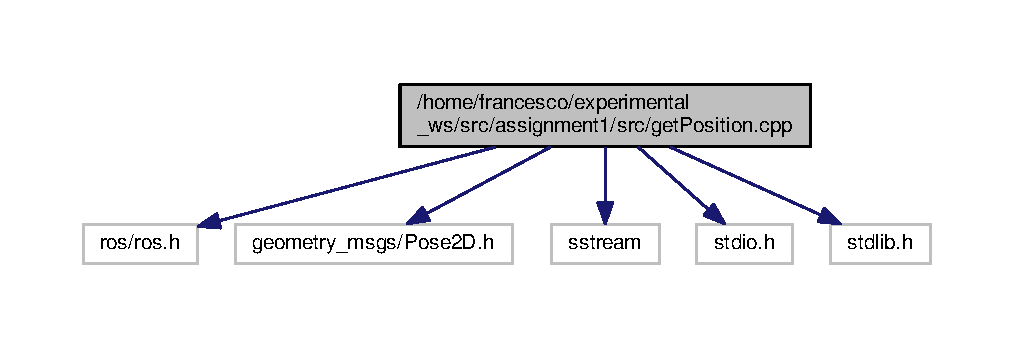
\includegraphics[width=350pt]{getPosition_8cpp__incl}
\end{center}
\end{figure}
\subsection*{Functions}
\begin{DoxyCompactItemize}
\item 
int \hyperlink{getPosition_8cpp_a3c04138a5bfe5d72780bb7e82a18e627}{main} (int argc, char $\ast$$\ast$argv)
\end{DoxyCompactItemize}


\subsection{Function Documentation}
\index{get\+Position.\+cpp@{get\+Position.\+cpp}!main@{main}}
\index{main@{main}!get\+Position.\+cpp@{get\+Position.\+cpp}}
\subsubsection[{\texorpdfstring{main(int argc, char $\ast$$\ast$argv)}{main(int argc, char **argv)}}]{\setlength{\rightskip}{0pt plus 5cm}int main (
\begin{DoxyParamCaption}
\item[{int}]{argc, }
\item[{char $\ast$$\ast$}]{argv}
\end{DoxyParamCaption}
)}\hypertarget{getPosition_8cpp_a3c04138a5bfe5d72780bb7e82a18e627}{}\label{getPosition_8cpp_a3c04138a5bfe5d72780bb7e82a18e627}
\hypertarget{State_8cpp_Description}{}\subsection{Description}\label{State_8cpp_Description}
This node publishes a random position which will be used from the command manager node. In practice it simulates the pointing gesture from the user and the random travel in N\+O\+R\+M\+AL mode as well. evry tiem we generate random position

at each iteration 
\hypertarget{Navigation_8cpp}{}\section{/home/francesco/experimental\+\_\+ws/src/assignment1/src/\+Navigation.cpp File Reference}
\label{Navigation_8cpp}\index{/home/francesco/experimental\+\_\+ws/src/assignment1/src/\+Navigation.\+cpp@{/home/francesco/experimental\+\_\+ws/src/assignment1/src/\+Navigation.\+cpp}}


It simulate the navigation from the current position to the position requested by the client, taking into account the dimension of a map a priori chosen.  


{\ttfamily \#include \char`\"{}ros/ros.\+h\char`\"{}}\\*
{\ttfamily \#include \char`\"{}assignment1/\+Go\+To.\+h\char`\"{}}\\*
Include dependency graph for Navigation.\+cpp\+:\nopagebreak
\begin{figure}[H]
\begin{center}
\leavevmode
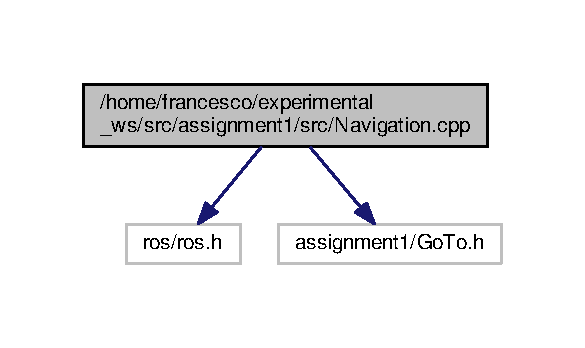
\includegraphics[width=281pt]{Navigation_8cpp__incl}
\end{center}
\end{figure}
\subsection*{Macros}
\begin{DoxyCompactItemize}
\item 
\#define \hyperlink{Navigation_8cpp_a8fd091040600c54e1b52be58d011ec30}{Xmax}~20
\begin{DoxyCompactList}\small\item\em Max dimension of the map along the X axis. \end{DoxyCompactList}\item 
\#define \hyperlink{Navigation_8cpp_aaf9edb39f963596bfe86fc184965dcb4}{Ymax}~20
\begin{DoxyCompactList}\small\item\em Max dimension of the map along the Y axis. \end{DoxyCompactList}\item 
\#define \hyperlink{Navigation_8cpp_a5e4cd1e773df9db61c1e224bc0872541}{homeX}~10
\begin{DoxyCompactList}\small\item\em X position of the House. \end{DoxyCompactList}\item 
\#define \hyperlink{Navigation_8cpp_af67938dd7cf91798c19150a38a90ddc8}{homeY}~20
\begin{DoxyCompactList}\small\item\em Y position of the House. \end{DoxyCompactList}\item 
\#define \hyperlink{Navigation_8cpp_a8cf66cab74089248cafe85e0ce12d9b3}{userX}~2
\begin{DoxyCompactList}\small\item\em X position of the user. \end{DoxyCompactList}\item 
\#define \hyperlink{Navigation_8cpp_abe6819b706873d83c9bd09343b28097f}{userY}~3
\begin{DoxyCompactList}\small\item\em Y position of the user. \end{DoxyCompactList}\end{DoxyCompactItemize}
\subsection*{Functions}
\begin{DoxyCompactItemize}
\item 
void \hyperlink{Navigation_8cpp_af65e9546a3cb9c4f867fbc597d5dc3cd}{printlogs} (int x, int y)
\item 
bool \hyperlink{Navigation_8cpp_aec33b62b66fc2284fabc2001b96599af}{go\+To} (assignment1\+::\+Go\+To\+::\+Request \&req, assignment1\+::\+Go\+To\+::\+Response \&res)
\item 
int \hyperlink{Navigation_8cpp_a3c04138a5bfe5d72780bb7e82a18e627}{main} (int argc, char $\ast$$\ast$argv)
\end{DoxyCompactItemize}


\subsection{Detailed Description}
It simulate the navigation from the current position to the position requested by the client, taking into account the dimension of a map a priori chosen. 

\hypertarget{State_8cpp_Description}{}\subsection{Description}\label{State_8cpp_Description}
\hypertarget{_}{}\subsubsection{}\label{_}
This service takes a X and Y positon request from the \char`\"{}command manager\char`\"{} node which is the only client. \begin{DoxySeeAlso}{See also}
\hyperlink{commandManager_8py}{command\+Manager.\+py} 
\end{DoxySeeAlso}


\subsection{Macro Definition Documentation}
\index{Navigation.\+cpp@{Navigation.\+cpp}!homeX@{homeX}}
\index{homeX@{homeX}!Navigation.\+cpp@{Navigation.\+cpp}}
\subsubsection[{\texorpdfstring{homeX}{homeX}}]{\setlength{\rightskip}{0pt plus 5cm}\#define homeX~10}\hypertarget{Navigation_8cpp_a5e4cd1e773df9db61c1e224bc0872541}{}\label{Navigation_8cpp_a5e4cd1e773df9db61c1e224bc0872541}


X position of the House. 

\index{Navigation.\+cpp@{Navigation.\+cpp}!homeY@{homeY}}
\index{homeY@{homeY}!Navigation.\+cpp@{Navigation.\+cpp}}
\subsubsection[{\texorpdfstring{homeY}{homeY}}]{\setlength{\rightskip}{0pt plus 5cm}\#define homeY~20}\hypertarget{Navigation_8cpp_af67938dd7cf91798c19150a38a90ddc8}{}\label{Navigation_8cpp_af67938dd7cf91798c19150a38a90ddc8}


Y position of the House. 

\index{Navigation.\+cpp@{Navigation.\+cpp}!userX@{userX}}
\index{userX@{userX}!Navigation.\+cpp@{Navigation.\+cpp}}
\subsubsection[{\texorpdfstring{userX}{userX}}]{\setlength{\rightskip}{0pt plus 5cm}\#define userX~2}\hypertarget{Navigation_8cpp_a8cf66cab74089248cafe85e0ce12d9b3}{}\label{Navigation_8cpp_a8cf66cab74089248cafe85e0ce12d9b3}


X position of the user. 

\index{Navigation.\+cpp@{Navigation.\+cpp}!userY@{userY}}
\index{userY@{userY}!Navigation.\+cpp@{Navigation.\+cpp}}
\subsubsection[{\texorpdfstring{userY}{userY}}]{\setlength{\rightskip}{0pt plus 5cm}\#define userY~3}\hypertarget{Navigation_8cpp_abe6819b706873d83c9bd09343b28097f}{}\label{Navigation_8cpp_abe6819b706873d83c9bd09343b28097f}


Y position of the user. 

\index{Navigation.\+cpp@{Navigation.\+cpp}!Xmax@{Xmax}}
\index{Xmax@{Xmax}!Navigation.\+cpp@{Navigation.\+cpp}}
\subsubsection[{\texorpdfstring{Xmax}{Xmax}}]{\setlength{\rightskip}{0pt plus 5cm}\#define Xmax~20}\hypertarget{Navigation_8cpp_a8fd091040600c54e1b52be58d011ec30}{}\label{Navigation_8cpp_a8fd091040600c54e1b52be58d011ec30}


Max dimension of the map along the X axis. 

\index{Navigation.\+cpp@{Navigation.\+cpp}!Ymax@{Ymax}}
\index{Ymax@{Ymax}!Navigation.\+cpp@{Navigation.\+cpp}}
\subsubsection[{\texorpdfstring{Ymax}{Ymax}}]{\setlength{\rightskip}{0pt plus 5cm}\#define Ymax~20}\hypertarget{Navigation_8cpp_aaf9edb39f963596bfe86fc184965dcb4}{}\label{Navigation_8cpp_aaf9edb39f963596bfe86fc184965dcb4}


Max dimension of the map along the Y axis. 



\subsection{Function Documentation}
\index{Navigation.\+cpp@{Navigation.\+cpp}!go\+To@{go\+To}}
\index{go\+To@{go\+To}!Navigation.\+cpp@{Navigation.\+cpp}}
\subsubsection[{\texorpdfstring{go\+To(assignment1\+::\+Go\+To\+::\+Request \&req, assignment1\+::\+Go\+To\+::\+Response \&res)}{goTo(assignment1::GoTo::Request &req, assignment1::GoTo::Response &res)}}]{\setlength{\rightskip}{0pt plus 5cm}bool go\+To (
\begin{DoxyParamCaption}
\item[{assignment1\+::\+Go\+To\+::\+Request \&}]{req, }
\item[{assignment1\+::\+Go\+To\+::\+Response \&}]{res}
\end{DoxyParamCaption}
)}\hypertarget{Navigation_8cpp_aec33b62b66fc2284fabc2001b96599af}{}\label{Navigation_8cpp_aec33b62b66fc2284fabc2001b96599af}
\hypertarget{Navigation.cpp_goTo}{}\subsection{go\+To}\label{Navigation.cpp_goTo}
This is the serve function which menages the requests from clients. It checks if the target position is within the map predefined by the parameters Xmax and Ymax if it is inside then it simulates the navigation simply waiting 3 seconds after which it assigns the request values to the response and sets to true the check variable. Otherwise it assigns false to the check variable\index{Navigation.\+cpp@{Navigation.\+cpp}!main@{main}}
\index{main@{main}!Navigation.\+cpp@{Navigation.\+cpp}}
\subsubsection[{\texorpdfstring{main(int argc, char $\ast$$\ast$argv)}{main(int argc, char **argv)}}]{\setlength{\rightskip}{0pt plus 5cm}int main (
\begin{DoxyParamCaption}
\item[{int}]{argc, }
\item[{char $\ast$$\ast$}]{argv}
\end{DoxyParamCaption}
)}\hypertarget{Navigation_8cpp_a3c04138a5bfe5d72780bb7e82a18e627}{}\label{Navigation_8cpp_a3c04138a5bfe5d72780bb7e82a18e627}
\index{Navigation.\+cpp@{Navigation.\+cpp}!printlogs@{printlogs}}
\index{printlogs@{printlogs}!Navigation.\+cpp@{Navigation.\+cpp}}
\subsubsection[{\texorpdfstring{printlogs(int x, int y)}{printlogs(int x, int y)}}]{\setlength{\rightskip}{0pt plus 5cm}void printlogs (
\begin{DoxyParamCaption}
\item[{int}]{x, }
\item[{int}]{y}
\end{DoxyParamCaption}
)}\hypertarget{Navigation_8cpp_af65e9546a3cb9c4f867fbc597d5dc3cd}{}\label{Navigation_8cpp_af65e9546a3cb9c4f867fbc597d5dc3cd}
\hypertarget{Navigation.cpp_printlogs}{}\subsection{printlogs}\label{Navigation.cpp_printlogs}
It\textquotesingle{}s a simple function that, based on the requested x y position, generates a log in the terminal 
\hypertarget{State_8cpp}{}\section{/home/francesco/experimental\+\_\+ws/src/assignment1/src/\+State.cpp File Reference}
\label{State_8cpp}\index{/home/francesco/experimental\+\_\+ws/src/assignment1/src/\+State.\+cpp@{/home/francesco/experimental\+\_\+ws/src/assignment1/src/\+State.\+cpp}}
{\ttfamily \#include \char`\"{}ros/ros.\+h\char`\"{}}\\*
{\ttfamily \#include \char`\"{}std\+\_\+msgs/\+String.\+h\char`\"{}}\\*
{\ttfamily \#include $<$sstream$>$}\\*
Include dependency graph for State.\+cpp\+:\nopagebreak
\begin{figure}[H]
\begin{center}
\leavevmode
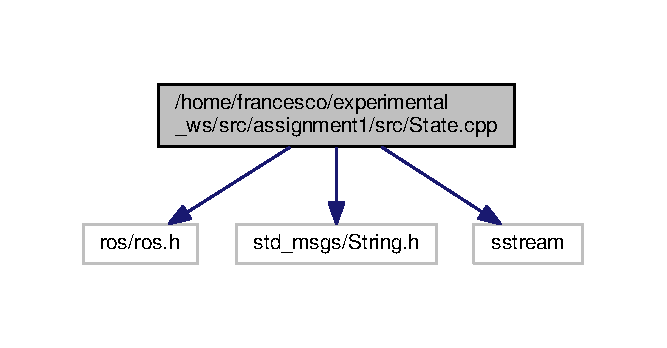
\includegraphics[width=320pt]{State_8cpp__incl}
\end{center}
\end{figure}
\subsection*{Functions}
\begin{DoxyCompactItemize}
\item 
int \hyperlink{State_8cpp_a3c04138a5bfe5d72780bb7e82a18e627}{main} (int argc, char $\ast$$\ast$argv)
\end{DoxyCompactItemize}


\subsection{Function Documentation}
\index{State.\+cpp@{State.\+cpp}!main@{main}}
\index{main@{main}!State.\+cpp@{State.\+cpp}}
\subsubsection[{\texorpdfstring{main(int argc, char $\ast$$\ast$argv)}{main(int argc, char **argv)}}]{\setlength{\rightskip}{0pt plus 5cm}int main (
\begin{DoxyParamCaption}
\item[{int}]{argc, }
\item[{char $\ast$$\ast$}]{argv}
\end{DoxyParamCaption}
)}\hypertarget{State_8cpp_a3c04138a5bfe5d72780bb7e82a18e627}{}\label{State_8cpp_a3c04138a5bfe5d72780bb7e82a18e627}
\hypertarget{State_8cpp_Description}{}\subsection{Description}\label{State_8cpp_Description}
This code generates a R\+OS node which is also a publisher. It publishes a string \textquotesingle{}play\textquotesingle{} on the topic Sate\+String. initialization of the variable which will randomly choose how often to generate a \textquotesingle{}play\textquotesingle{} message

choose randomly the next time iteration 
\hypertarget{state__machine_8py}{}\section{/home/francesco/experimental\+\_\+ws/src/assignment1/src/state\+\_\+machine.py File Reference}
\label{state__machine_8py}\index{/home/francesco/experimental\+\_\+ws/src/assignment1/src/state\+\_\+machine.\+py@{/home/francesco/experimental\+\_\+ws/src/assignment1/src/state\+\_\+machine.\+py}}
\subsection*{Classes}
\begin{DoxyCompactItemize}
\item 
class \hyperlink{classstate__machine_1_1Unlocked}{state\+\_\+machine.\+Unlocked}
\item 
class \hyperlink{classstate__machine_1_1Locked}{state\+\_\+machine.\+Locked}
\end{DoxyCompactItemize}
\subsection*{Namespaces}
\begin{DoxyCompactItemize}
\item 
 \hyperlink{namespacestate__machine}{state\+\_\+machine}
\end{DoxyCompactItemize}
\subsection*{Functions}
\begin{DoxyCompactItemize}
\item 
def \hyperlink{namespacestate__machine_afaa99f0eebff6571a958fcc827c6a367}{state\+\_\+machine.\+user\+\_\+action} ()
\item 
def \hyperlink{namespacestate__machine_a5c680ce705e6052fa07c6cece21743d0}{state\+\_\+machine.\+main} ()
\end{DoxyCompactItemize}

%--- End generated contents ---

% Index
\backmatter
\newpage
\phantomsection
\clearemptydoublepage
\addcontentsline{toc}{chapter}{Index}
\printindex

\end{document}
